\documentclass[10pt, conference, a4paper, final]{IEEEtran}
\IEEEoverridecommandlockouts
% For better handling of math expressions
\usepackage{amsmath}

% For better formatting of lists
\usepackage{enumitem}
\usepackage{amssymb}
% Optional for improved typography
\usepackage{microtype}
\usepackage[margin=1in]{geometry} % Adjust margins as needed
\usepackage{lipsum} % Provides sample text. Remove this for your actual document.
\usepackage[table,xcdraw]{xcolor}
\usepackage{colortbl}
\usepackage{graphicx} % Required for including images
\usepackage{graphicx}
\usepackage{textcomp}
\usepackage{xcolor}
\usepackage{float}
\usepackage{amsmath}
\usepackage{longtable}
\usepackage{booktabs}
\usepackage{multicol}
\usepackage{multirow}
\usepackage{relsize, fullpage, url, array}
\usepackage{lscape, afterpage}
\usepackage{float,lscape}
\usepackage{algorithm}
\usepackage{algorithmic}  
\usepackage[algo2e]{algorithm2e} 
\usepackage{amsmath}
\usepackage{mathtools}
\usepackage{tabularx}
\usepackage{algorithmic}
\usepackage{graphicx}
\usepackage{textcomp}
\usepackage{xcolor}
\usepackage{subcaption}

\title{Uncovering Adversarial Vulnerabilities in Deep Learning: A Shapley Value-Based Approach for Detailed Pixel Analysis}
\author{Arooj Arif}
\date{\today} % You can also specify a date manually

\begin{document}

\maketitle % This command creates the title


\begin{abstract}    
    Adversarial attacks in the deep learning domain significantly threaten model transparency and robustness. Adversarial perturbations are unnoticeable for humans. Hence, it is necessary to develop methods of counteracting these attacks. In this research, we present a new way to use SHAP (SHapley Additive exPlanations) to analyze image pixels at a finer level. We thoroughly investigate four adversarial attacks, carefully studying their effects on model vulnerability by analyzing their impact at different epsilon values. Our approach focuses on identifying crucial pixels in image-based model, uncovering vulnerabilities, and enhancing model robustness through SHAP analysis. This extensive study provides valuable insights for the development of AI systems that are more secure and transparent. These findings have important implications in critical healthcare and autonomous driving areas. Our research solves existing problems with AI security and establishes new benchmarks for how AI systems can combine robustness with interpretability.
\end{abstract}

\section{Introduction}

Deep learning is becoming increasingly important and is now a vital component of modern computational applications. It uses multiple layers to process data and create computational models, introducing various algorithms such as generative adversarial networks, convolutional neural networks, and model transfers. These algorithms have revolutionized the way we process information and have shown significant progress in domains such as visual, audio, and text processing, social network analysis, and natural language processing. It has also successfully addressed challenges in machine learning such as unsupervised and online learning. Its ability to handle massive and complex datasets has made it a critical tool for extensive data analysis. Compared to traditional machine learning approaches, its state-of-the-art performance has led to its widespread adoption in fields such as image processing, computer vision, speech recognition, machine translation, medical imaging, and many others.\cite {Saad, Md}. In today's world, with the rapid advancements and widespread adoption of technology, it has become crucial to focus on the strength and reliability of deep learning models. These models are increasingly being used in critical safety and socially significant applications like autonomous driving, face recognition, and malware detection, where their efficiency and dependability are of utmost importance. However, deep neural networks have been found to be susceptible to both adversarial and natural image detection that can significantly impact their performance. By exploring and improving the robustness of these models, we can ensure their effectiveness and reliability in real-world scenarios \cite {Numair, Aleksandar}.

Adversarial attacks present a unique challenge for deep learning models. They exploit subtle weaknesses, causing misclassification of examples with imperceptible changes. Such attacks can have a severe impact on the reliability and safety of deep learning models, especially in safety-critical applications like autonomous driving. Adversarial examples can lead to incorrect decisions, potentially resulting in severe consequences. Therefore, it is crucial to analyze the robustness and reliability of deep learning models to ensure their safety in real-world deployments \cite {Samuel, Muhammad}. 
Explainable Artificial Intelligence (XAI) is a critical component in addressing the challenges of deep learning. It helps to enhance the understanding and trustworthiness of AI by providing interpretable and human-understandable explanations of AI decisions. The techniques, tools, and algorithms used in XAI generate explanations that help build trustworthy and interpretable deep learning models. These explanations improve trust by providing insights into the model's decision-making process, addressing challenges of trust, transparency, bias understanding, and fairness, and promoting a more robust and impartial decision-making process \cite {Mohammed, Aha, Tamer}. 

Despite recent advancements in deep learning models, research has identified gaps and shortcomings in making these models robust against adversarial attacks. It has been observed that there is an overly disproportionate focus on adversarial machine learning compared to non-adversarial robustness. Additionally, there is a significant gap in model performance when faced with naturally-induced image corruptions or alterations, which can result in performance degradation similar to that seen in adversarial conditions. This vulnerability to natural image corruptions suggests that understanding model performance on natural data should be prioritized before focusing on resilience to adversarial attack scenarios \cite {Numair, Tianhang, Wei}. 

We conducted a research to explore the challenges posed by adversarial attacks on deep learning models. Our primary focus was on understanding and quantifying the impacts of different pixels. To achieve this, we used SHAP (SHapley Additive exPlanations) within the realm of Explainable Artificial Intelligence (XAI) to unravel the complex dynamics of how deep learning models respond to adversarial manipulations. Our goal was not only to identify vulnerabilities but also to enhance the robustness and transparency of these models. The stakes are high in critical applications such as healthcare and autonomous systems. Therefore, our research strives to fortify these models against adversarial threats while simultaneously improving their interpretability and trustworthiness. Through this work, we aim to bridge the existing gap between robustness and transparency in AI, offering novel insights and methodologies that could significantly advance the field.

\section{Contributions of the Paper}

This paper introduces several significant contributions to the field of AI, particularly in enhancing the robustness and transparency of deep learning models against adversarial threats:

\begin{itemize}
    \item \textbf{Novel Integration of SHAP-based XAI in Adversarial Analysis:} Our work pioneers the application of SHAP-based critical pixel analysis, offering a new perspective in understanding and mitigating these threats at a pixel level.
    
    \item \textbf{Comprehensive Evaluation of Model Behavior:} By employing the MNIST dataset across a range of adversarial intensities, our research provides a detailed assessment of model vulnerabilities, crucial for developing more resilient AI systems.
    
    \item \textbf{Insightful Analysis through Advanced Visualization:} Utilizing UMAP visualizations, our study reveals intricate patterns and impacts of adversarial attacks, enhancing the interpretability of complex model behaviors in a user-friendly manner.
    
    \item \textbf{In-depth Contrastive Analysis of SHAP Values:} Our research conducts a thorough comparison of SHAP values between normal and adversarial examples, shedding light on the subtle ways adversarial attacks influence model decision-making.
    
    \item \textbf{Statistical Validation of Model Vulnerabilities:} We introduce a rigorous statistical approach to validate the significance of identified vulnerabilities, thereby strengthening the reliability of our findings and setting a new standard in adversarial robustness research.

\end{itemize}

\section{Background and Related Work}

\subsection{Model Architecture and Output Formulation of Deep Neural Networks}



The following is an explanation of a deep neural network classification model denoted by \( F(\cdot) : \mathbb{R}^d \rightarrow [0, 1]^{C} \). Its purpose is to take an image with dimensions \( d = h \times w \times c \) and classify it into one of several categories (output labels) with a probability vector \( F(x) \) of dimensions \( C \). The input to the model is an image vector, and the output is a probability distribution of all possible labels, where \( F(x)_i \)  is the probability that the input vector \( x \)  is labeled with \( i \). 

The Logits of the final layer of a Deep Neural Network (DNN) is represented by \(L(\cdot)\), and the model output is calculated by using the softmax activation function on Logits. This can be expressed as \cite {ZhangS.}:

\begin{equation}
    F(x) = \text{softmax}(L(x)).
    \end{equation}

The label with the highest probability in \( F(x) \) is the predicted label of an input image \( x \), and it looks like this \cite {ZhangS.}: 
\begin{equation}
    \hat{y} = \arg\max_i (F(x)_i).
    \end{equation}

Let's assume that the deep neural network has \( l + 1 \) layers, with the input layer being the 0-th layer and the output layer being the \( l \)-th layer. The output of the \( i \)-th neural network layer is denoted as \( F_i(\cdot) \).

\subsection{Adversarial Attacks and Defense Mechanisms} 

The process used to create adversarial samples is called an adversarial attack model. It involves using a model, denoted by  \( F(\cdot) \), and an original input image, denoted by \( x \), to create an adversarial sample, denoted by \( x' = x + d \) , by introducing a specific perturbation to \( x \). This perturbation, denoted by \( d \), causes the model to predict a different label for the adversarial sample \( x' \) than it would for the original sample \( x \) \cite {ZhangS.}.

\begin{align}
    \hat{y}' &\neq \hat{y}, \\
    \text{where } \hat{y} &= \arg\max_i (F(x)_i) \text{and} \\
    \hat{y}'&= \arg\max_i (F(x')_i),
\end{align}

The perturbation \( \|d\| < \epsilon \) must have an absolute value less than epsilon, where epsilon represents the maximum perturbation size. The distance metric, denoted by  \( \|\cdot\| \) , is used to measure the perturbation, which can be quantified by three norms: \( l_0 \), \( l_2 \), and 
\( l_{\infty} \). The \( l_0 \) norm counts the number of altered non-zero elements, or the number of pixels that have been modified by the adversarial attack in the original image. The \( l_2 \) norm refers to the conventional Euclidean distance, which is obtained by summing the squares of the modified elements and then taking the square root. The \( l_{\infty} \) norm represents the highest value among all the elements of the perturbation. Recently, Wang et al. (34) used a novel distance metric that relies on Just Noticeable Distortion (JND) to more accurately assess the perceptual similarity and provide adversarial instances that are more visually realistic. By default, this article uses the 
\( l_{\infty} \) norm to quantify the magnitude of the disturbance.

Several techniques for generating adversarial examples have been developed in recent years. Some of the most prominent options that we utilize for our assessment include:


\subsubsection{Fast Gradient Sign Method (FGSM) \cite {Goodfellow.}}

Adversarial samples are generated by the Fast Gradient Sign Method (FGSM), which utilizes the linear properties of deep neural networks. In this method, the adversarial example \( x' \) is obtained by :
\begin{equation}
    x' = x + \epsilon \cdot \text{sign}(\nabla_x J(x, y));
\end{equation}

Here, \( x \) represents the original image, \( x' \) represents the adversarial example, \( J \) refers to the loss function, and \( \epsilon \) is the perturbation limit. This technique modifies the pixels uniformly based on the gradient of the loss function.



\subsubsection{Basic Iterative Method (BIM) \cite {Kurakin., Madry.}}

The Basic Iterative Method (BIM), proposed by Alexey and colleagues, is an extension of the FGSM method that progressively improves upon it. In each step, a minor disturbance is introduced by the following equation: 
\begin{equation}
    x'_{i} = \text{clip}_{x, \epsilon} \left( x'_{i-1} + \epsilon \cdot \text{sign}(\nabla_{x'_{i-1}} L(x'_{i-1}, y)) \right);
    \end{equation}
The BIM algorithm starts with an initial value of \( x'_0 = x \), and a clipping function is applied to ensure that the modified image remains within specified boundaries. The iterative nature of this method enables more precise fine-tuning compared to the FGSM method.


\subsubsection{Projected Gradient Descent (PGD) \cite {Stiff}}

PGD, an extension of FGSM, adopts a multi-step approach:
\begin{equation}
x'_0 = x \quad 
\end{equation}
\begin{equation}
x'_{t+1} = \text{clip}_{[0,1]} \left( x'_t + \alpha \cdot \text{sign}(\nabla J_\theta(x'_t, l)) \right)
\end{equation}
The \(\text{clip}_{[0,1]}(\cdot)\) function ensures the perturbed image remains within [0, 1]. PGD is computationally intensive but offers a stronger and more precise attack than FGSM.



Projected Gradient Descent (PGD) is a technique that is derived from the Fast Gradient Sign Method (FGSM).
\begin{equation}
    x'_0 = x \quad 
    \end{equation}
    \begin{equation}
    x'_{t+1} = \text{clip}_{[0,1]} \left( x'_t + \alpha \cdot \text{sign}(\nabla J(\theta, x'_t, l)) \right)
    \end{equation}

The perturbed image is then clipped to the range of [0,1] using the function \(\text{clip}_{[0,1]}(\cdot)\). This process is performed until a certain number of iterations is reached. The PGD algorithm requires a significant amount of computational resources, but it provides a more robust and accurate method of attack compared to the FGSM.


\subsubsection{DeepFool}

DeepFool \cite {Moosavi} is an algorithm that aims to generate adversarial examples with minimal perturbation. The algorithm minimizes the \(L_2\) norm and iteratively applies small perturbations to an input image using a linear neural network. 

The objective of DeepFool is to find the smallest perturbation required to change the classification of an input image. The algorithm computes the perturbation by solving the following optimization problem:

\begin{equation}
r^*(x_0) = \arg\min_r \|r\| \quad \text{s.t.} \quad \text{sign}(f(x_0 + r)) \neq \text{sign}(f(x_0)),
\end{equation}

The solution to this problem can be approximated using the gradient of the neural network. When the gradient is not available, DeepFool uses an approximation based on the linearization of the neural network. The perturbation is computed as follows:

\begin{equation}
r^*(x_0) = \frac{|f(x_0)|}{\|w\|^2} w.
\end{equation}

DeepFool can also be used to generate targeted adversarial examples. In this case, the algorithm solves the following optimization problem:

\begin{equation}
\arg\min_{r_i} \|r_i\|^2 \quad \text{s.t.} \quad f(x_i) + \nabla f(x_i)^T r_i = 0.
\end{equation}

DeepFool has been shown to be effective in generating adversarial examples with comparable accuracy to FGSM but with less perturbation.

According to the research \cite {Ilyas.}, the existence of adversarial examples in a dataset is an intrinsic property. The authors introduce the concept of robust and non-robust characteristics to classify dataset features. Non-robust features exhibit high predictive power but also exhibit high susceptibility to significant changes when slight perturbations are introduced to the input. Conversely, robust features possess high predictive power and are resistant to slight changes in the input. Robust features are considered as fundamental aspects of the target class, such as the presence of wheels and windows in cars. Non-robust features are seemingly arbitrary patterns that are not easily discernible by humans but demonstrate strong predictive power during the training phase. The work of \cite {Ilyas.} illustrates that non-robust features play a significant role in the generation of adversarial examples and their ability to move between different classification models. These non-robust features are vulnerable to minor perturbations in the input, which can result in significant changes in the value of these highly predictive features.

Some examples of defense methods against adversarial example include adversarial training \cite {Goodfellow.}, Defensive Distillation \cite {Papernot}, Gradient Obfuscation, Feature Squeezing \cite {Evans}, ML-LOO \cite {Yang}, Density Estimates \cite {Feinman}, Local Intrinsic Dimensionality \cite {Ma}, Mahalanobis Distance 
 \cite {Lee}, and many more. In our research, we propose a method for identifying critical pixels in both normal and adversarial examples. This will aid in the generation and defense of attacks. 


\subsection{Explainable AI}

Explainable AI (XAI) plays a crucial role in the field of machine learning as it enables AI systems to be transparent and comprehensible. Its main objective is to establish confidence and effectively handle complex AI solutions. The role of XAI is particularly important in supervised models as it enables a comprehensive explanation of the reasoning behind predictions. Prominent XAI techniques include LIME \cite {Ribeiro}, which provides localized explanations of predictions, DeepLIFT \cite {Shrikumar}, which tracks the contributions of individual neurons, and SHAP \cite {LundbergandS}, which employs Shapley values derived from game theory to evaluate the influence of each input on model decisions, particularly advantageous in anomaly identification.

Our research focuses on DeepExplainer \cite{LundbergandS} that is extension of SHAP, a specialized tool developed exclusively for deep neural networks (DNNs). DeepExplainer integrates the Shapley value and DeepLIFT techniques to enhance computing efficiency and provide clear and intuitive explanations. It is widely used in various domains such as engineering \cite{Mangalathu}, aerospace \cite{Aouf}, medical \cite{Singh},  transportation \cite{Parsa}, manufacturing \cite{Huang}, security \cite{Warnecke}, and others due to its ability to analyze complex models. 

DeepSHAP has proven to be crucial in detecting adversarial examples. It is used in image detection to differentiate between adversarial and normal samples, as well as for identifying word-level adversarial attacks. Our study expands the applicability of SHAP values beyond being just a general XAI indicator. Instead, we use SHAP values to specifically pinpoint crucial pixels, thus increasing our understanding of adversarial attack manipulations and strengthening the resilience of AI models.




\section{Proposed Methodology:}

\begin{figure*}[!ht]
    \centering
    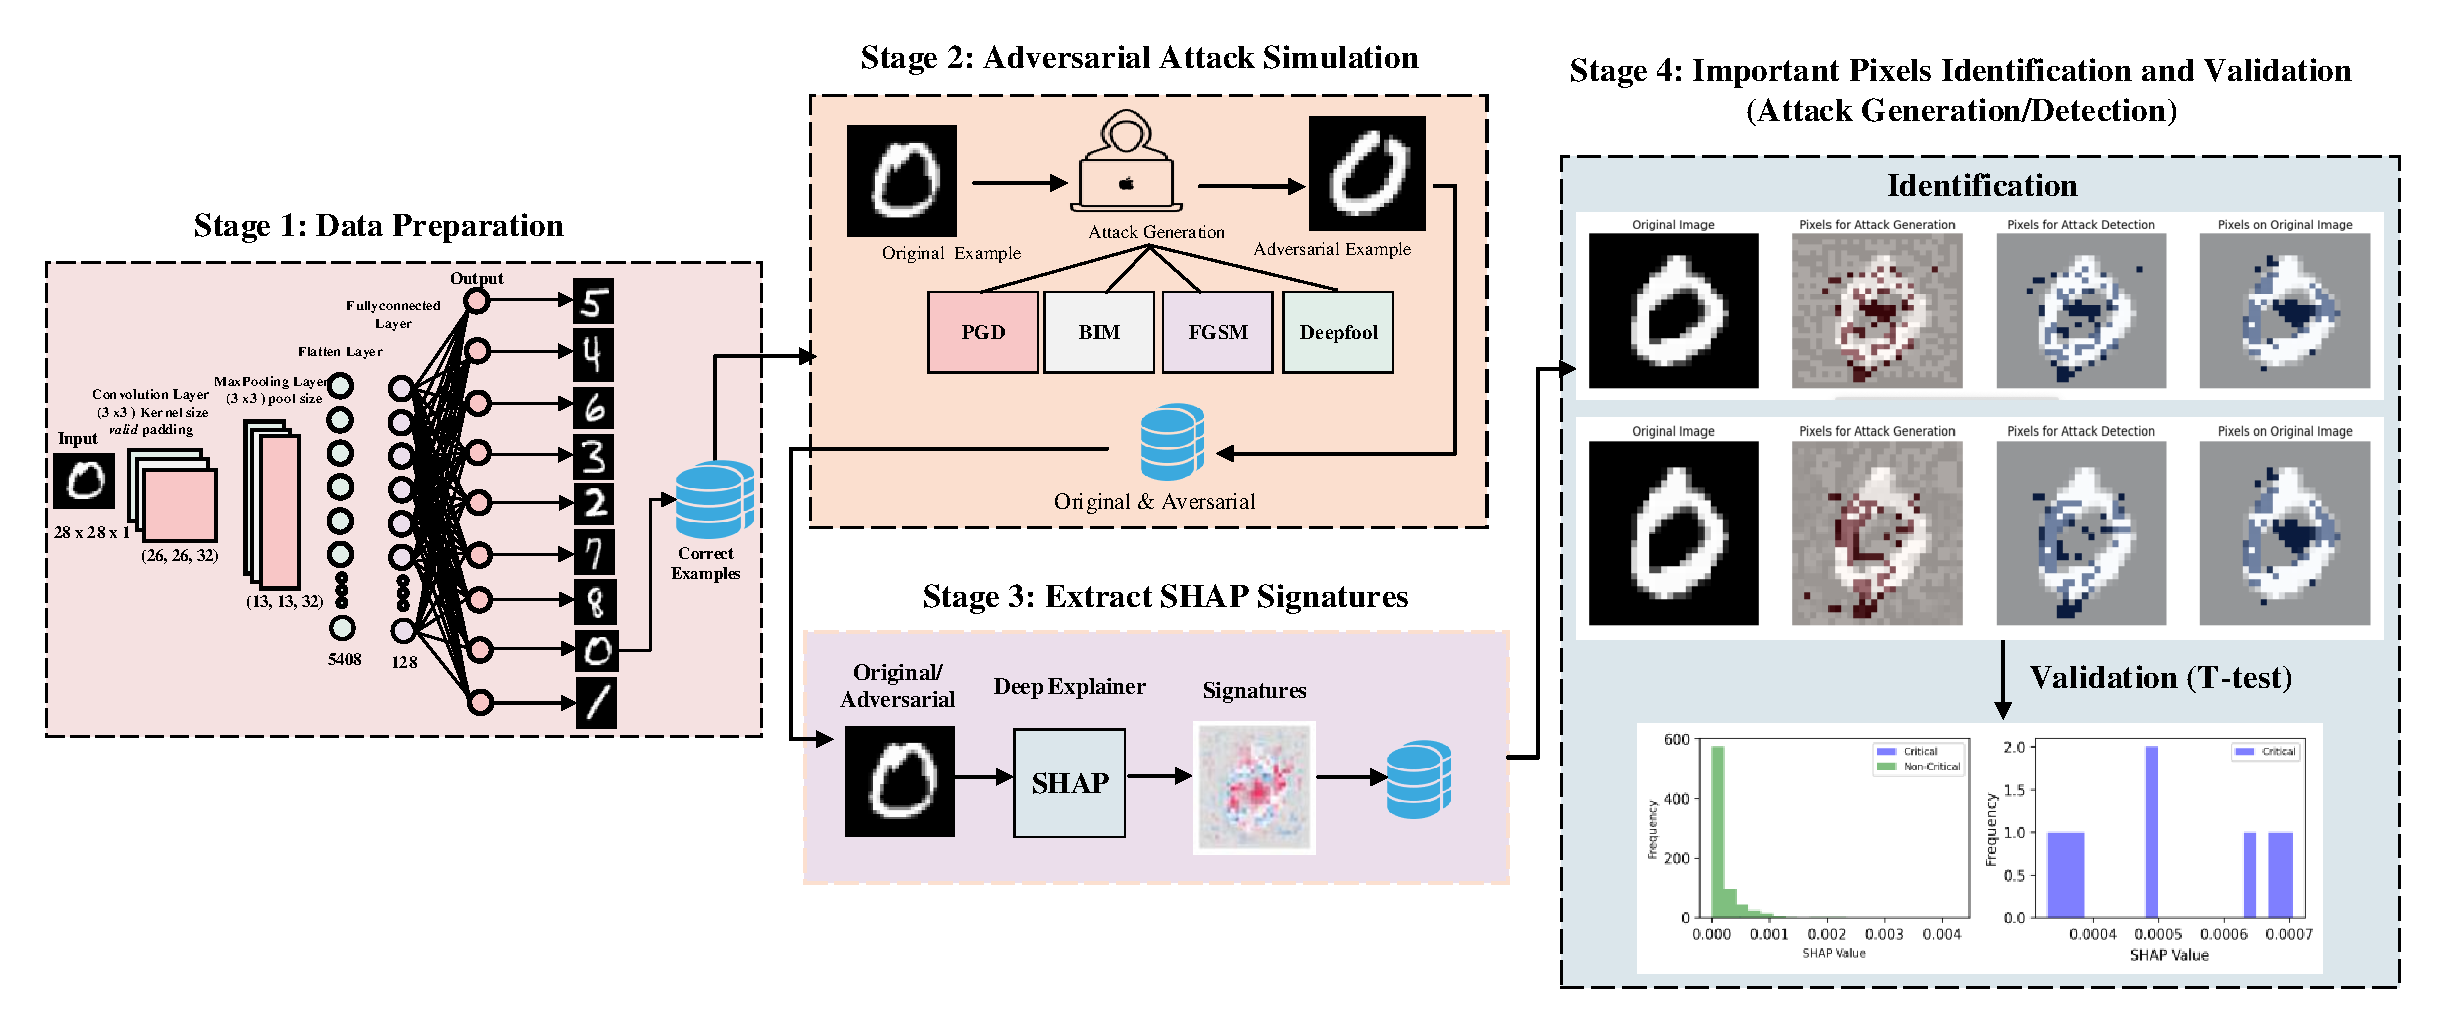
\includegraphics[width=1\textwidth]{paper_images/model.pdf}
    \caption{Overview of the Proposed Model}
    \label{overview}
\end{figure*}
   
Our research, illustrated in Figure. \ref{overview}, aims to improve the defense strategies of deep learning systems against complex attacks. We accomplish this by training Convolutional Neural Networks with the MNIST dataset and focusing on correctly identifying images. To test the strength of our model, we carry out a series of sophisticated simulated attacks to challenge the system's decision-making abilities in different scenarios. We then conduct a comprehensive analysis to determine the effect of each step size on the model's decision-making process, particularly during these simulated attacks. In the final phase, we use a specialized technique to identify the most critical pixels in attack generation and detection scenarios. Additionally, we employ a statistical method called the t-test to evaluate and confirm the significance of these identified critical points. This process ensures the accuracy and dependability of our findings. Our model's multi-stage, comprehensive approach protects against a wide range of adversarial threats in deep learning environments.


\subsection{Stage 1: Data and Model Preparation}

In the initial stage of our investigation, we used CNN, which had already been trained on the MNIST dataset, to classify digits. A crucial step prior to the study was to carefully select cases that the model could accurately classify, resulting in a dataset comprising only correctly predicted instances. This aimed to help us understand how adversarial perturbations impact a model performing well otherwise.
We chose a dataset with a varied class distribution that accurately reflected real-world scenarios. The dataset consisted of 973 instances labeled as 0, 1133 as 1, 1016 as 2, 989 as 3, 969 as 4, 882 as 5, 937 as 6, 1005 as 7, 946 as 8, and 984 as 9. Although the digit frequencies were not perfectly uniform, we acknowledged this slight imbalance to ensure the integrity of our study. Rather than using a synthetically balanced environment, we wanted to test the model's ability to counter adversarial attacks in a real-world scenario. This approach allowed us to focus on the model's robustness in situations it would encounter in the real world.

To ensure that our study focused on how adversarial attacks impact a model already performing well, we focused on accurately classified cases. Our systematic methodology in data selection formed a well-defined foundation for our investigation, enabling us to examine the ability of neural networks to tolerate adversarial manipulations in a way that closely resembles real-world scenarios.


\subsection{Stage 2: Adversarial Attack Simulation}

In the previous stage, we created adversarial examples to test how reliable the model is. Our objective was to evaluate the performance of the neural network model when it is exposed to misleading conditions deliberately. We chose a range of epsilon values, which were set to [0.03, 0.04, 0.05, 0.1, 0.2, 0.25], to create different levels of disturbance intensities.

Through this approach, we could comprehensively examine how the model reacted to different degrees of adversarial intensity. This is essential to determine its overall robustness. We used Foolbox, a Python library, to aid in creating a broad range of adversarial attacks.

We executed various types of adversarial attacks, including LinfBasicIterativeAttack (BIM), LinfFastGradientAttack (FGSM), LinfDeepFoolAttack, and LinfProjectedGradientDescentAttack (PGD). We systematically gathered and analyzed the adversarial examples created from these attacks.
Figure. \ref{fig:umap} shows a UMAP visualization of the MNIST dataset, where each point represents a digit from 0 to 9. The colors represent the original digit classes, while the adversarial examples produced by PGD attacks are interspersed within these clusters. This visualization helps us understand how adversarial perturbations affect classification accuracy and identify vulnerabilities in the model. By gaining insights from this analysis, we can improve the model's defense and ensure its reliability against adversarial threats in practical scenarios.


\begin{figure*}[!ht]
    \centering
    \begin{subfigure}{.50\textwidth}
        \centering
        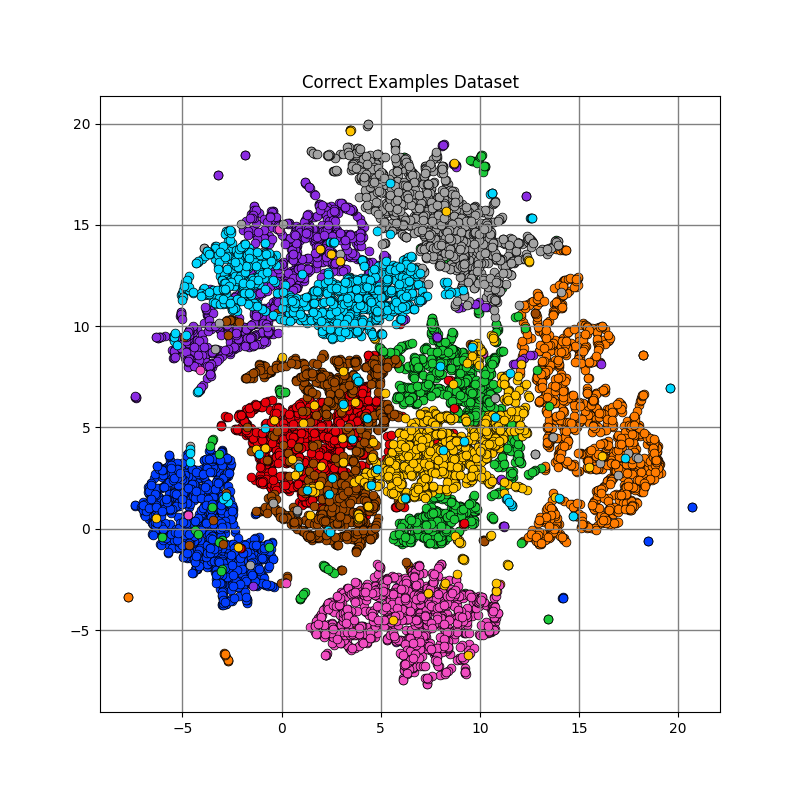
\includegraphics[width=\linewidth]{paper_images/1.png}
        \caption{Original MNIST digit classes}
        \label{fig:umap_original}
    \end{subfigure}%
    \hfill
    \begin{subfigure}{.50\textwidth}
        \centering
        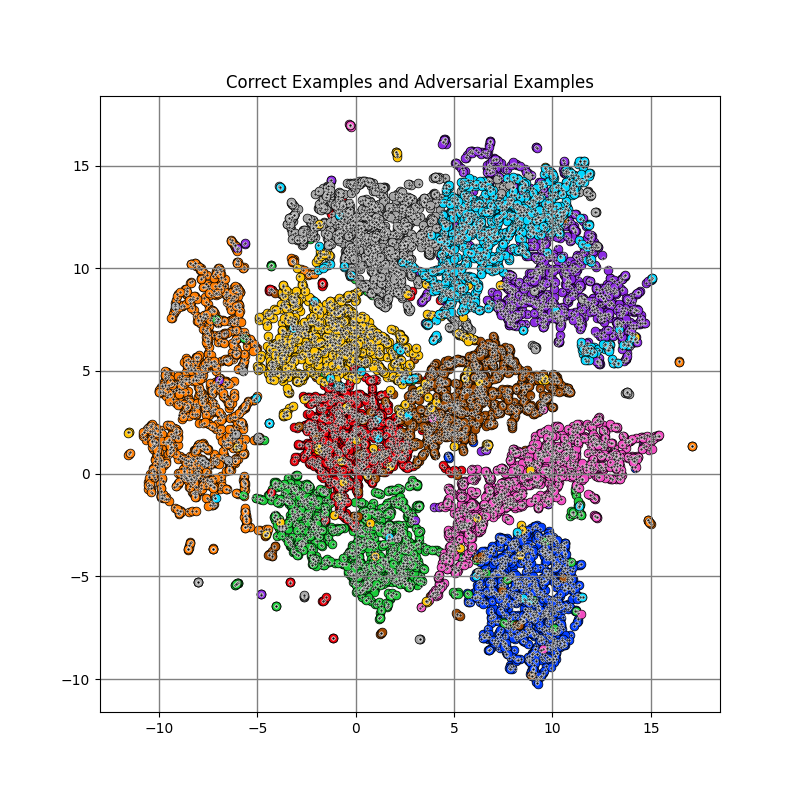
\includegraphics[width=\linewidth]{paper_images/2.png}
        \caption{Original and PGD attack}
        \label{fig:umap_pgd}
    \end{subfigure}
    \caption{UMAP projections illustrating the separation of digit classes within the MNIST dataset and the integration of adversarial examples.
     The left panel (\ref{fig:umap_original}) shows the natural clustering of MNIST digits, and the right panel panel (\ref{fig:umap_pgd}) overlays PGD 
     adversarial examples.}
    \label{fig:umap}
\end{figure*}



\subsection{Stage 3: Extraction of XAI Signatures}
In this stage, we aimed to analyze the influence of input pixels on model predictions. We examined both standard and adversarial altered data. We used Deep Explainer to highlight the contribution of each pixel towards the model's output. By calculating SHAP values for specific subsets of our data, we could compare the effect of standard inputs versus adversarial inputs. This approach helped us identify significant differences in their influence on the model's predictions. It allowed us to gain valuable insights into the model's decision-making process when presented with adversarial conditions.

\begin{figure}[h]
\centering
\begin{subfigure}{\columnwidth}
\centering
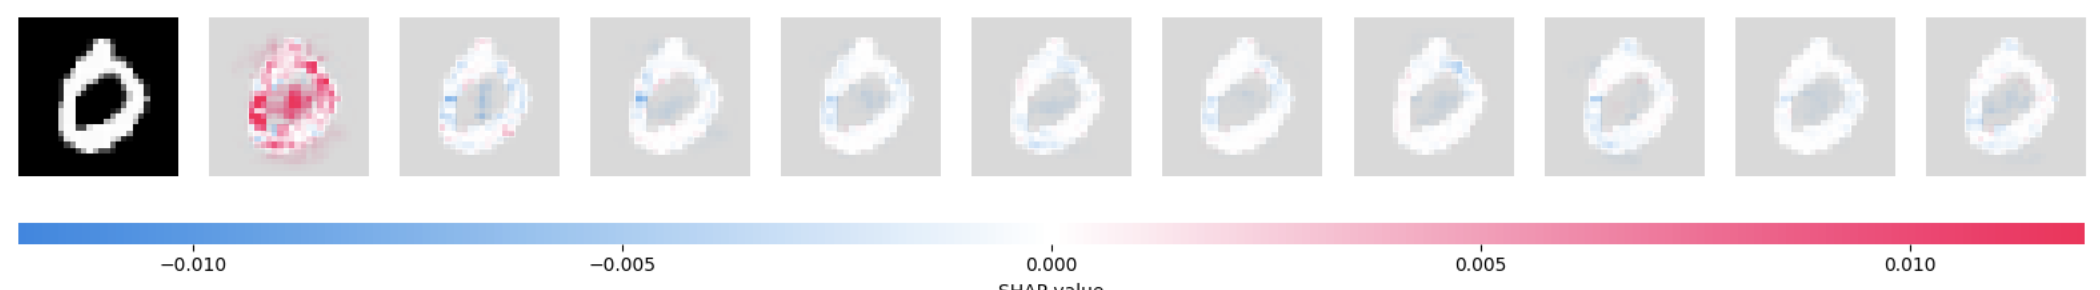
\includegraphics[width=\linewidth]{paper_images/normal.png}
\label{fig:correct_shap}
\end{subfigure}
\par\medskip
\begin{subfigure}{\columnwidth}
\centering
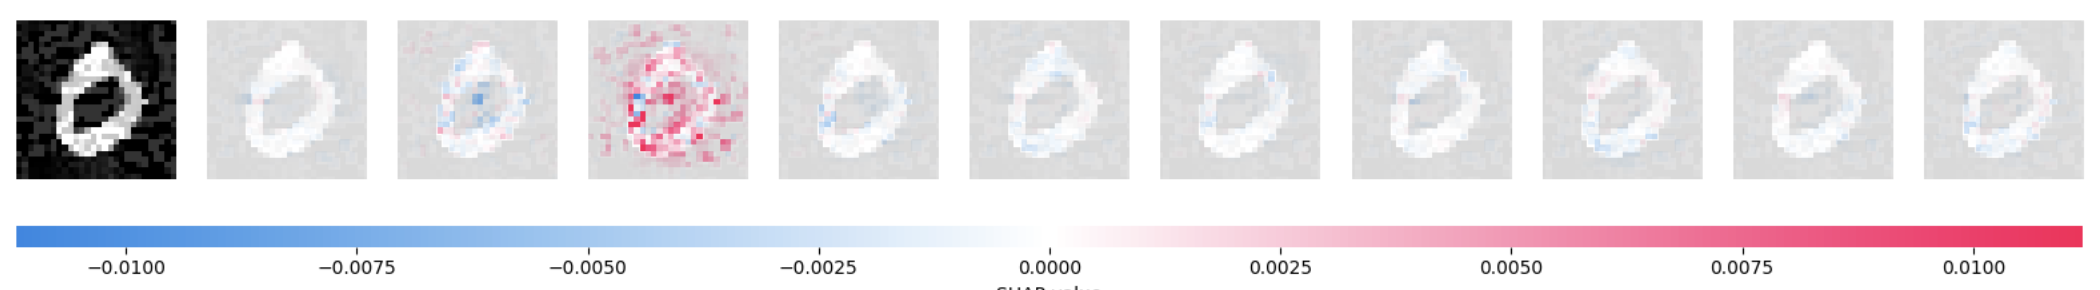
\includegraphics[width=\linewidth]{paper_images/pgd.png}
\label{fig:pgd}
\end{subfigure}
\begin{subfigure}{\columnwidth}
\centering
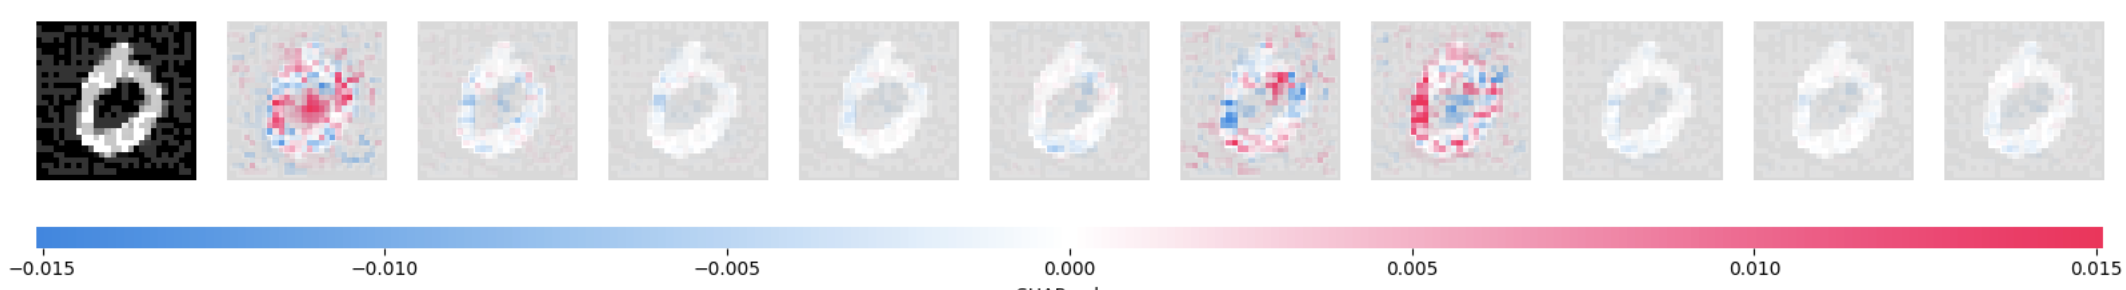
\includegraphics[width=\linewidth]{paper_images/fgsm.png}
\label{fig:fgsm}
\end{subfigure}
\begin{subfigure}{\columnwidth}
\centering
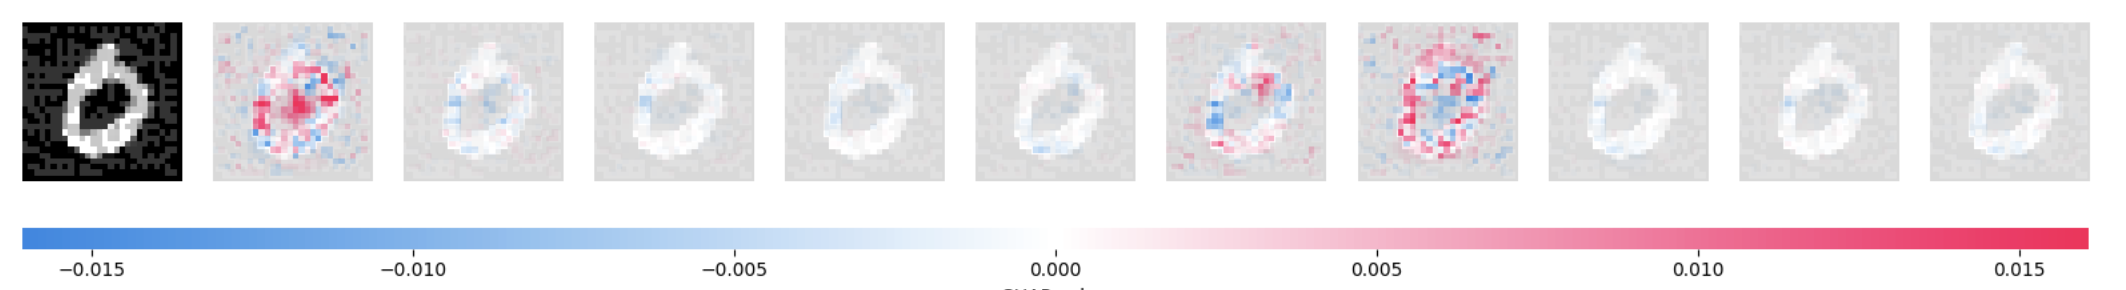
\includegraphics[width=\linewidth]{paper_images/deep.png}
\label{fig:deep}
\end{subfigure}
\begin{subfigure}{\columnwidth}
\centering
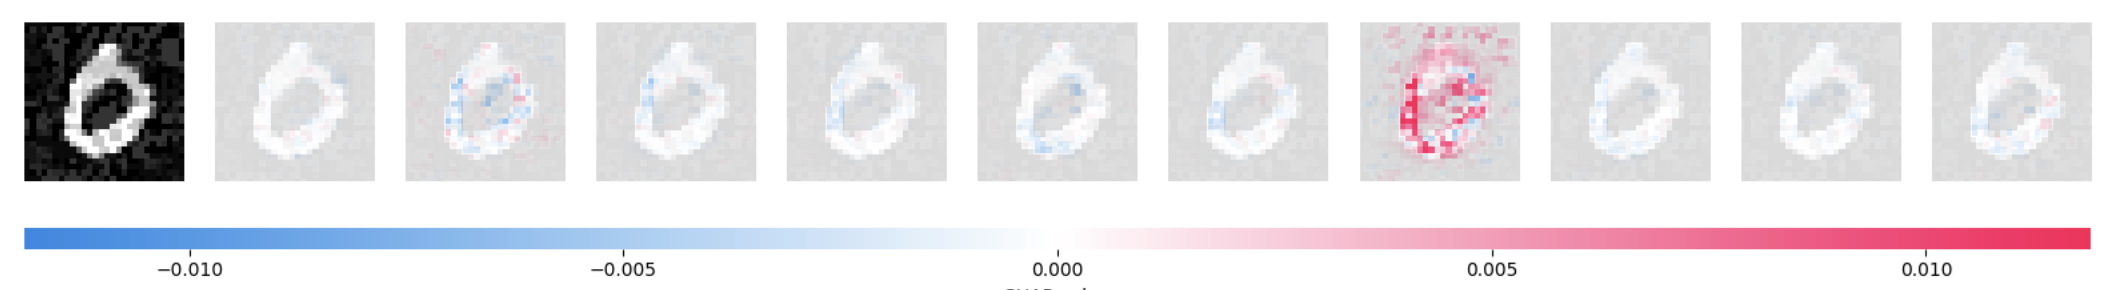
\includegraphics[width=\linewidth]{paper_images/basic.png}
\label{fig:basic}
\end{subfigure}
\caption{SHAP heatmaps depicts the interpretability of a model's decision for a normally classified digit and its progressive alteration under various adversarial attacks (PGD, FGSM, deepfool and basic iterative method), highlighting the shift in influential pixels at a granular level. (a): Normal, (b): PGD, (c): FGSM, (d): Deep Fool, (e): BIM}
\label{fig:both_shap_figures}
\end{figure}



    
\section{Stage 4: Identification and Validation of Critical Pixels}

\subsection{SHAP Values for Critical Pixel Analysis}
    In Stage 4, we use the SHAP values that we extracted earlier to pinpoint and confirm the pixels that have a significant impact on the 
    model's predictions. This step is essential for gaining a deeper understanding of the model's behavior and developing effective strategies 
    to make it more resilient to adversarial attacks.
    The process involves:

 \subsubsection{Attack Generation Pixel Analysis}
We first analyze the SHAP values for adversarial image pixels. This step is crucial to identify which pixels, when altered, are most effective 
in generating successful adversarial attacks. By understanding the pixels that significantly influence the model's erroneous decisions, we can 
uncover how adversarial perturbations are guided and how they can be strategically crafted.

\subsubsection{Attack Detection Pixel Analysis}
Subsequently, we focus on detecting these adversarial manipulations by examining the differences in SHAP values between normal and adversarial
images. This comparison highlights the pixels where the largest deviations occur, signaling potential areas of the image being exploited by 
adversarial attacks. This analysis is vital for developing robust detection mechanisms that can identify and counteract these manipulative 
changes.

\subsubsection{Original Image Pixel Importance}
Alongside these analyses, we also scrutinize the SHAP values of original, unmanipulated images. This examination is essential to establish a 
baseline of the model’s interpretation of unperturbed images. Understanding the importance of pixels in the original context provides a 
reference point, helping us to better interpret the changes observed in the adversarial context.

Through this comprehensive methodology, we aim to provide a deep understanding of how pixel-level manipulations affect AI decision-making, 
both in generating and detecting adversarial attacks, as well as understanding the inherent behavior of the model under normal conditions.

\subsubsection{Statistical Validation of Critical Pixels}
To substantiate the distinction between critical and non-critical pixels identified in our analysis, we conducted a statistical t-test on the
 SHAP values. This test helps validate the significance of the differences observed in the SHAP values between critical and non-critical pixels.
  The implementation of a t-test ensures that the observed disparities are not due to random chance, thereby lending statistical rigor to our 
  findinßgs and confirming the reliability of our pixel importance assessments.


    
    \begin{figure}[h]
        \centering
        \begin{subfigure}{\columnwidth}
            \centering
            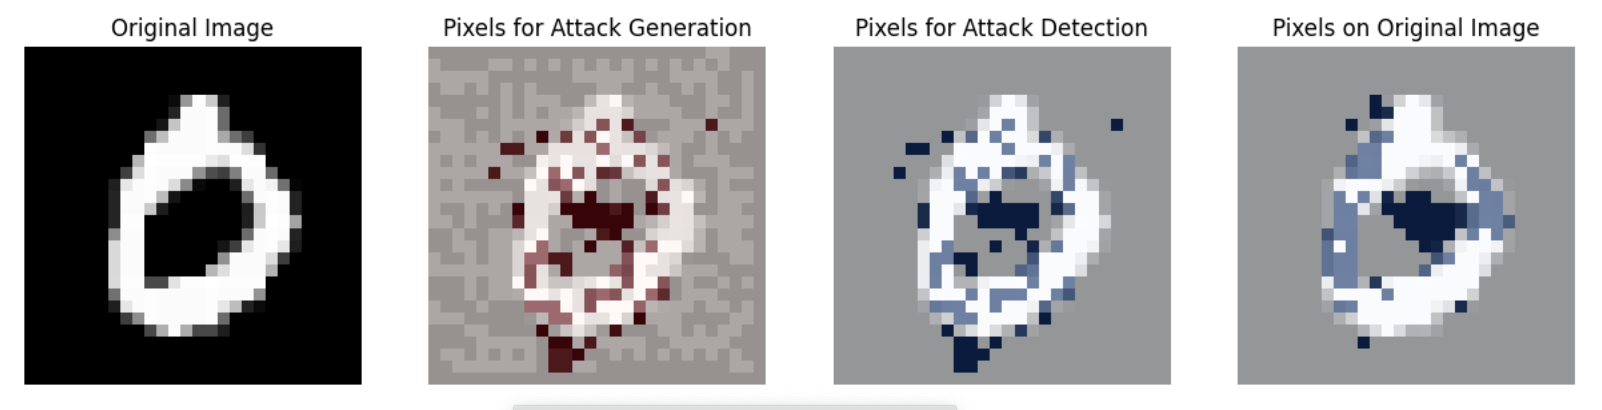
\includegraphics[width=\linewidth]{paper_images/fgsm_c.png}
            \caption{FGSM}
            \label{fig:fgsm_c}
        \end{subfigure}
        \par\medskip % Adds space between the two subfigures
        \begin{subfigure}{\columnwidth}
            \centering
            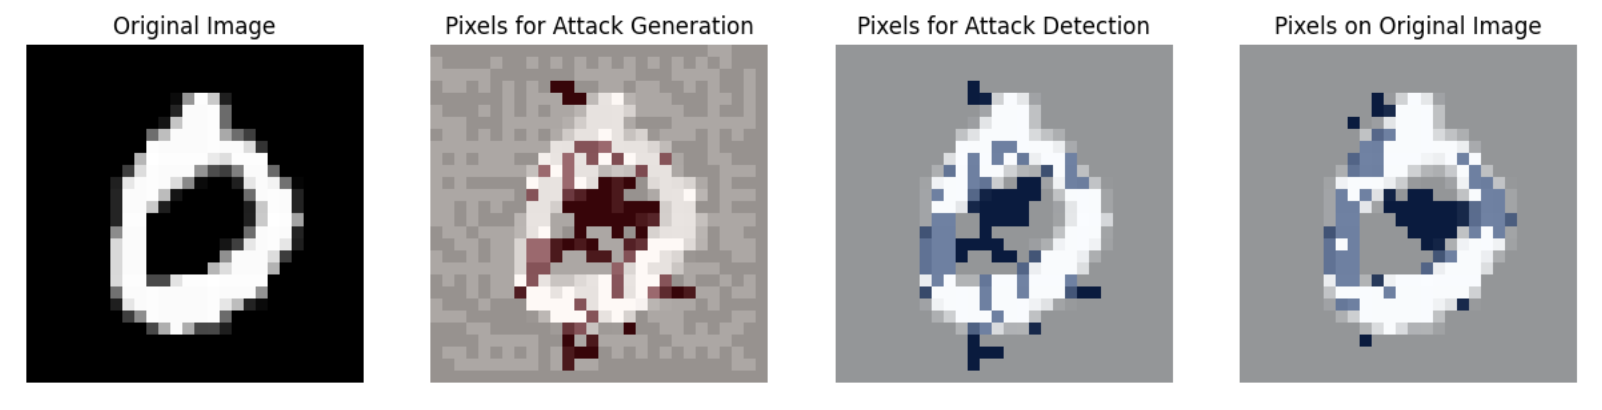
\includegraphics[width=\linewidth]{paper_images/deep_c.png}
            \caption{Deepfool}
            \label{fig:deep_c}
        \end{subfigure}
        \begin{subfigure}{\columnwidth}
            \centering
            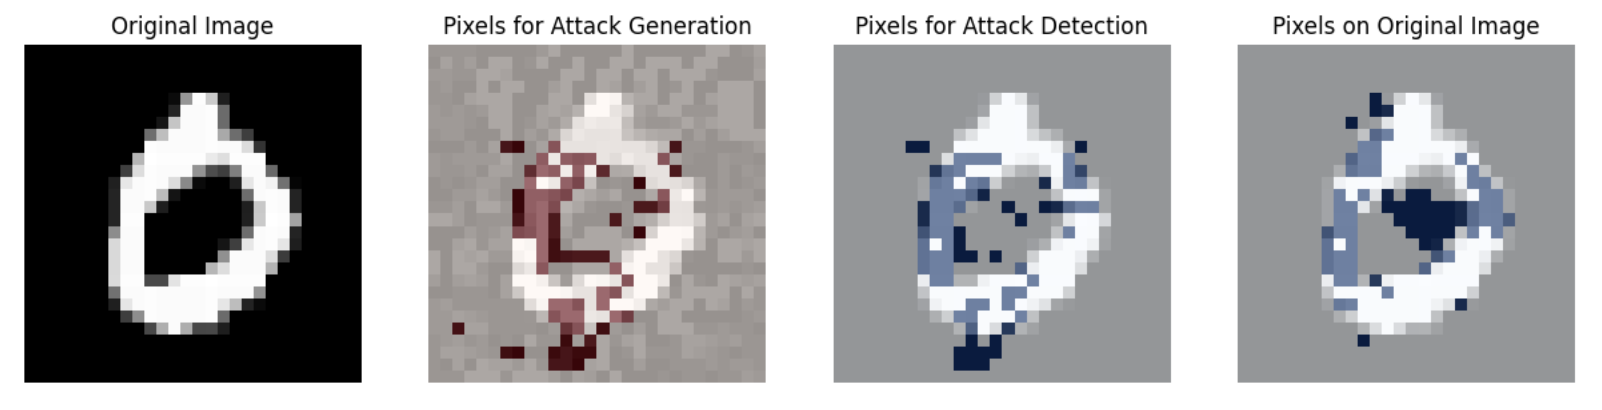
\includegraphics[width=\linewidth]{paper_images/basic_c.png}
            \caption{Basic Iterative Method}
            \label{fig:fgsm}
        \end{subfigure}
        \begin{subfigure}{\columnwidth}
            \centering
            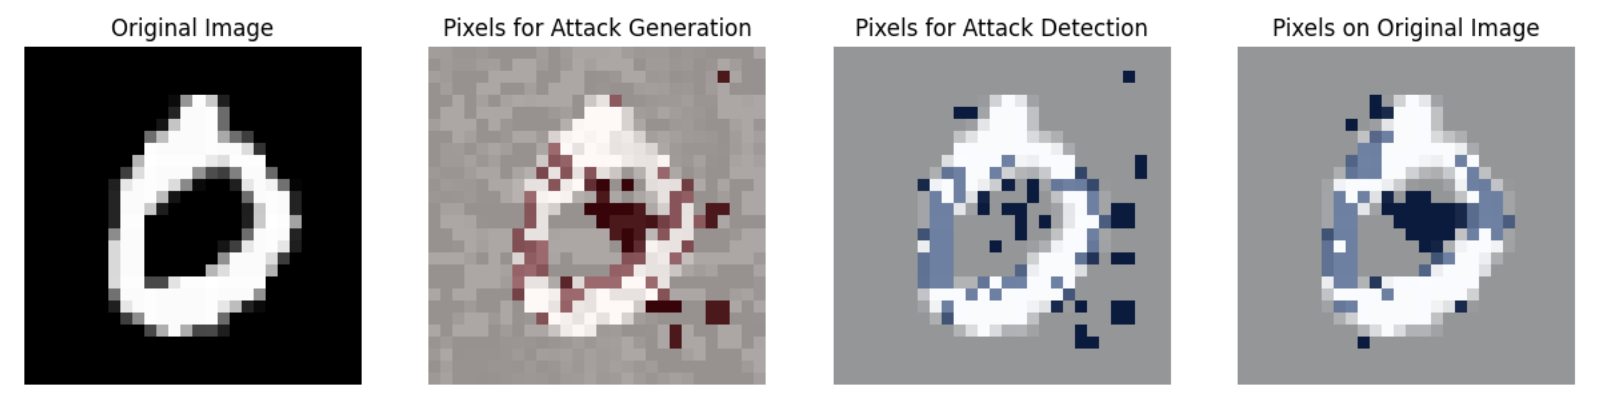
\includegraphics[width=\linewidth]{paper_images/pgd_c.png}
            \caption{PGD}
            \label{fig:deep}
        \end{subfigure}
     
        \caption{Visualization of critical pixels in adversarial samples.}
        \label{fig:both_shap_figures}
    \end{figure}
    
    \begin{table*}[t]
        \centering
        \begin{tabular}{|p{3cm}|p{6cm}|}
        \hline
        \textbf{SHAP Value Proximity to Zero} & \textbf{Interpretation} \\ \hline
        Close to Zero & 
        \begin{itemize}
        \item Feature has minimal impact on the model's prediction.
        \item Changes in the feature value do not significantly affect the prediction.
        \item Feature is considered neutral or weak in terms of prediction influence.
        \end{itemize}
        \\ \hline
        Far from Zero (Positive or Negative) & 
        \begin{itemize}
        \item Feature has a substantial impact on the model's prediction.
        \item Variations in the feature value lead to significant changes in the prediction.
        \item Feature is a strong influencer of the predicted outcome.
        \item The magnitude of the SHAP value indicates the strength of the feature's influence.
        \end{itemize}
        \\ \hline
        \end{tabular}
        \caption{Interpretations of SHAP Values Based on Proximity to Zero}
        \label{table:shap-value-interpretation}
    \end{table*}
    
    

% In Stage 5 of our research, we focused on the development of a binary classification model that could effectively differentiate between original and adversarial examples. The crux of this stage was the utilization of XAI signatures, particularly SHAP values, instead of raw data. The choice of XAI signatures was strategic and stemmed from the need for deeper insights into the decision-making processes of neural networks. These signatures, unlike raw data, provide a nuanced understanding of feature importance and contributions, making them immensely valuable in identifying subtle manipulations in adversarial examples.

% This approach aligns with the broader objective of enhancing the interpretability and trustworthiness of deep learning models. By using XAI signatures, we aim to gain a more transparent view into how and why models make certain decisions, especially under adversarial conditions. This transparency is crucial for identifying potential vulnerabilities and strengthening the model's defenses against sophisticated attacks.

% Moreover, understanding the influence of individual features on model predictions through XAI signatures aids significantly in the research and development of more robust attack detection methods. It enables us to pinpoint which features are most exploited in adversarial attacks and thus devise more effective strategies to counter them.

% For the testing phase, we opted for a simple neural network model. This choice was deliberate; a simpler model allows for clearer interpretation of results and a more straightforward evaluation of the effectiveness of XAI signatures. It serves as a preliminary testing ground, where we can assess the viability of our approach before scaling up to more complex models. This step is essential in ensuring that our methodology is sound and effective in a controlled environment before applying it to more intricate and real-world scenarios.
% Evaluate the classification model's performance in correctly identifying adversarial attacks.

\section{Experiments:}

In our evaluation we aimed to answer the following two research questions:
\begin{itemize}
    \item\textbf{RQ1:} How effective is SHapley Additive exPlanations (SHAP) analysis in identifying specific pixel-level vulnerabilities in deep learning models, and what insights does it provide for understanding the nature of these vulnerabilities?
    \item\textbf{RQ2:} In what ways can the findings from SHAP-based fine-grained pixel analysis be applied to enhance the robustness of deep learning models against sophisticated adversarial attacks?
\end{itemize}
\subsection{Case Study 1: Evaluating Model Robustness Against Different Adversarial Attacks}

The main objective of this case study is to evaluate the robustness of the MNIST classification model 
against different kinds of adversarial attacks such as Basic Iterative Method (BIM), Fast Gradient Sign Method (FGSM), 
DeepFool, and Projected Gradient Descent (PGD). The focus of the study is to compare the performance of the MNIST model
before and after being subjected to these adversarial attacks. The performance will be measured by the number of misclassifications
that occur at different levels of perturbation, as measured by the epsilon values. The study aims to provide insights into the
vulnerabilities of the MNIST model to different types of adversarial attacks and to determine the effectiveness of these attacks 
at varying intensities. Figure \ref {fig:robust_accuracy_attacks} represents the model's accuracy against various types of attacks. 
The graph shows how the accuracy of the model decreases with the increasing intensity of the perturbation, which is measured by epsilon.
This trend of decreasing robust accuracy is observed for all types of attacks.



\begin{figure}[ht]
    \centering
    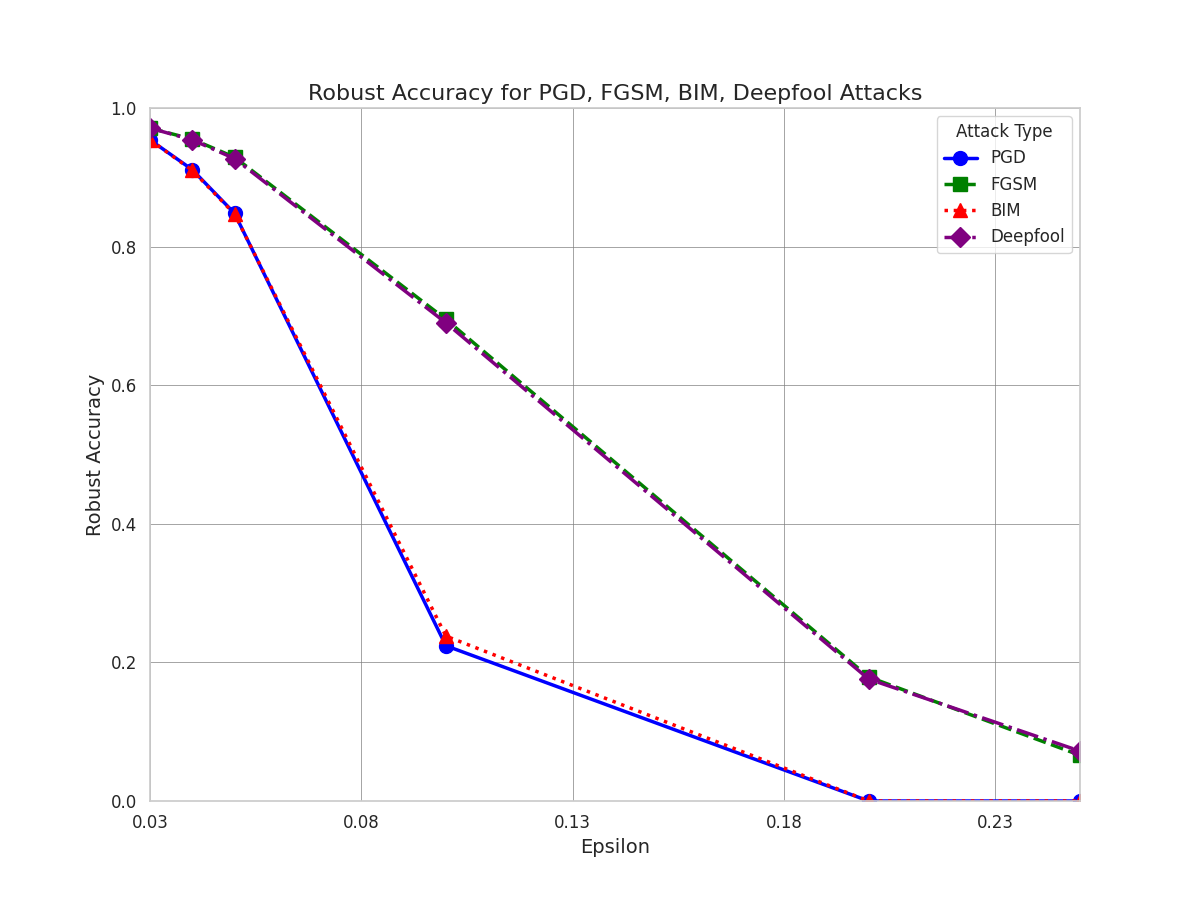
\includegraphics[width=\linewidth]{paper_images/robust.png}
    \caption{Relation between attacks (PGD, FGSM, BIM, Deepfool) success rate and Perturbation size}
    \label{fig:robust_accuracy_attacks}
\end{figure}


\begin{table}[ht]
    \centering
    \caption{Summary of Total Misclassifications for Various Adversarial Attacks}
    \label{tab:misclassifications}
    \begin{tabular}{|l|c|c|c|c|c|c|}
    \hline
    & \multicolumn{6}{c|}{\textbf{Epsilon}} \\ \cline{2-7} 
    \multirow{-2}{*}{\textbf{Attack Type}} & \textbf{0.03} & \textbf{0.04} & \textbf{0.05} & \textbf{0.10} & \textbf{0.20} & \textbf{0.25} \\ \hline
    BIM & 451 & 881 & 1508 & 7490 & 9834 & 9834 \\ \hline
    FGSM & 284 & 440 & 702 & 2998 & 8070 & 9186 \\ \hline
    Deepfool & 289 & 449 & 713 & 3045 & 8104 & 9130 \\ \hline
    PGD & 451 & 881 & 1483 & 7616 & 9834 & 9834 \\ \hline
    \end{tabular}
\end{table}

The findings emphasize the importance of implementing advanced defensive measures to enhance the robustness of machine learning models against 
adversarial attacks. The observations made in this case study can help in the creation of such defenses, especially in addressing the weaknesses exposed by BIM and PGD when dealing with smaller perturbations, and the slower but eventual impact of FGSM and DeepFool when dealing with higher perturbations.

\subsection{Critical Analysis of Class-Specific Metrics}

In the field of adversarial machine learning, it's important to evaluate how well a model performs when faced with attacks. While overall metrics like robust accuracy and misclassification rates give a general idea of a model's performance, it's important to also examine class-specific metrics like F1-Score, Precision, and Recall. These metrics help to identify specific vulnerabilities in the model, especially in a security context where false positives and false negatives can have different implications. To get a more detailed understanding of the model's performance, we've compiled a table Table. \ref{table2} that shows the F1-Score, Precision, and Recall for each class under different types of attacks and perturbations. This table not only demonstrates the model's overall resilience but also highlights specific weaknesses in certain classes that may be overlooked in more general analyses.

As an example, high precision rate during an attack indicates that when a model predicts a specific class, it is likely accurate, although it may miss out on identifying all true instances (resulting in lower recall). On the other hand, high recall with low precision suggests a model that is prone to false alarms by classifying non-members as belonging to the targeted class. The F1-Score metric balances precision and recall to provide a single measure.

Upon careful analysis of the table, it has been observed that certain classes are more susceptible to specific types of attacks. This highlights the necessity of implementing targeted defensive strategies for these classes. For instance, classes that exhibit a significant drop in F1-Score when attacked with FGSM are particularly vulnerable to the perturbations caused by this method. This knowledge can inform the creation of tailored training data or the implementation of defense mechanisms specific to these classes.
Furthermore, the variation in robustness between classes can guide the allocation of defense resources. Classes with lower robustness metrics represent weak points in the model's defenses and could benefit from focused defense measures.
In conclusion, the comprehensive evaluation of the model's robustness provided by the detailed metrics, robust accuracy trends, and misclassification insights in the table is essential in developing effective defenses against adversarial attacks. This multifaceted assessment ensures that the model remains accurate and trustworthy in the face of ever-evolving adversarial challenges.

    \begin{table}[ht]
        \centering
        \resizebox{\columnwidth}{!}{%
        \begin{tabular}{cccccccccccccc}
        \toprule
        Epsilon & Class & \multicolumn{12}{c}{Metrics} \\
        \cmidrule(lr){3-14}
         & & \rotatebox{90}{F1-Score BIM} & \rotatebox{90}{F1-Score Deepfool} & \rotatebox{90}{F1-Score FGSM} & \rotatebox{90}{F1-Score PGD} & \rotatebox{90}{Precision BIM} & \rotatebox{90}{Precision Deepfool} & \rotatebox{90}{Precision FGSM} & \rotatebox{90}{Precision PGD} & \rotatebox{90}{Recall BIM} & \rotatebox{90}{Recall Deepfool} & \rotatebox{90}{Recall FGSM} & \rotatebox{90}{Recall PGD} \\
        \midrule
        0.03 & 0 & 0.9842 & 0.9872 & 0.9872 & 0.9842 & 0.9777 & 0.9817 & 0.9817 & 0.9777 & 0.9908 & 0.9928 & 0.9928 & 0.9908 \\
        0.03 & 1 & 0.9690 & 0.9788 & 0.9792 & 0.9664 & 0.9454 & 0.9601 & 0.9609 & 0.9444 & 0.9938 & 0.9982 & 0.9982 & 0.9894 \\
        0.03 & 2 & 0.9446 & 0.9675 & 0.9669 & 0.9442 & 0.9405 & 0.9694 & 0.9693 & 0.9396 & 0.9488 & 0.9656 & 0.9646 & 0.9488 \\
        0.03 & 3 & 0.9612 & 0.9778 & 0.9783 & 0.9627 & 0.9588 & 0.9749 & 0.9749 & 0.9589 & 0.9636 & 0.9808 & 0.9818 & 0.9666 \\
        0.03 & 4 & 0.9558 & 0.9717 & 0.9722 & 0.9573 & 0.9519 & 0.9692 & 0.9712 & 0.9548 & 0.9598 & 0.9742 & 0.9732 & 0.9598 \\
        0.03 & 5 & 0.9557 & 0.9715 & 0.9726 & 0.9544 & 0.9349 & 0.9571 & 0.9582 & 0.9357 & 0.9773 & 0.9864 & 0.9875 & 0.9739 \\
        0.03 & 6 & 0.9693 & 0.9796 & 0.9801 & 0.9693 & 0.9793 & 0.9860 & 0.9870 & 0.9783 & 0.9594 & 0.9733 & 0.9733 & 0.9605 \\
        0.03 & 7 & 0.9455 & 0.9682 & 0.9682 & 0.9459 & 0.9498 & 0.9682 & 0.9663 & 0.9517 & 0.9413 & 0.9682 & 0.9701 & 0.9403 \\
        0.03 & 8 & 0.9233 & 0.9464 & 0.9480 & 0.9234 & 0.9731 & 0.9807 & 0.9830 & 0.9720 & 0.8784 & 0.9144 & 0.9154 & 0.8795 \\
        0.03 & 9 & 0.9289 & 0.9550 & 0.9560 & 0.9301 & 0.9351 & 0.9619 & 0.9619 & 0.9335 & 0.9227 & 0.9482 & 0.9502 & 0.9268 \\
        0.04 & 0 & 0.9708 & 0.9826 & 0.9821 & 0.9718 & 0.9664 & 0.9766 & 0.9757 & 0.9693 & 0.9753 & 0.9887 & 0.9887 & 0.9743 \\
        0.04 & 1 & 0.9432 & 0.9708 & 0.9716 & 0.9367 & 0.9071 & 0.9464 & 0.9479 & 0.9026 & 0.9823 & 0.9965 & 0.9965 & 0.9735 \\
        0.04 & 2 & 0.8994 & 0.9461 & 0.9471 & 0.8980 & 0.8840 & 0.9424 & 0.9434 & 0.8822 & 0.9154 & 0.9498 & 0.9508 & 0.9144 \\
        0.04 & 3 & 0.9192 & 0.9596 & 0.9611 & 0.9185 & 0.9124 & 0.9577 & 0.9597 & 0.9081 & 0.9262 & 0.9616 & 0.9626 & 0.9292 \\
        0.04 & 4 & 0.9098 & 0.9568 & 0.9579 & 0.9116 & 0.8984 & 0.9529 & 0.9539 & 0.9028 & 0.9216 & 0.9607 & 0.9618 & 0.9205 \\
        0.04 & 5 & 0.8995 & 0.9546 & 0.9546 & 0.9010 & 0.8550 & 0.9320 & 0.9320 & 0.8614 & 0.9490 & 0.9785 & 0.9785 & 0.9444 \\
        0.04 & 6 & 0.9373 & 0.9698 & 0.9703 & 0.9402 & 0.9587 & 0.9804 & 0.9814 & 0.9579 & 0.9167 & 0.9594 & 0.9594 & 0.9232 \\
        0.04 & 7 & 0.9073 & 0.9512 & 0.9513 & 0.9042 & 0.9141 & 0.9521 & 0.9494 & 0.9162 & 0.9005 & 0.9502 & 0.9532 & 0.8925 \\
        0.04 & 8 & 0.8493 & 0.9163 & 0.9202 & 0.8527 & 0.9491 & 0.9704 & 0.9751 & 0.9447 & 0.7685 & 0.8679 & 0.8710 & 0.7770 \\
        0.04 & 9 & 0.8548 & 0.9304 & 0.9314 & 0.8586 & 0.8729 & 0.9371 & 0.9390 & 0.8721 & 0.8374 & 0.9238 & 0.9238 & 0.8455 \\
        0.05 & 0 & 0.9532 & 0.9750 & 0.9750 & 0.9559 & 0.9546 & 0.9686 & 0.9686 & 0.9549 & 0.9517 & 0.9815 & 0.9815 & 0.9568 \\
        0.05 & 1 & 0.9095 & 0.9534 & 0.9542 & 0.9031 & 0.8583 & 0.9169 & 0.9177 & 0.8538 & 0.9673 & 0.9929 & 0.9938 & 0.9585 \\
        0.05 & 2 & 0.8318 & 0.9189 & 0.9198 & 0.8318 & 0.8061 & 0.9118 & 0.9136 & 0.8105 & 0.8593 & 0.9262 & 0.9262 & 0.8543 \\
        0.05 & 3 & 0.8496 & 0.9311 & 0.9321 & 0.8532 & 0.8215 & 0.9260 & 0.9279 & 0.8292 & 0.8797 & 0.9363 & 0.9363 & 0.8787 \\
        0.05 & 4 & 0.8547 & 0.9300 & 0.9325 & 0.8589 & 0.8390 & 0.9143 & 0.9180 & 0.8481 & 0.8710 & 0.9463 & 0.9474 & 0.8700 \\
        0.05 & 5 & 0.8297 & 0.9208 & 0.9214 & 0.8325 & 0.7735 & 0.8825 & 0.8827 & 0.7838 & 0.8946 & 0.9626 & 0.9637 & 0.8878 \\
        0.05 & 6 & 0.8966 & 0.9533 & 0.9555 & 0.9047 & 0.9361 & 0.9701 & 0.9724 & 0.9402 & 0.8602 & 0.9370 & 0.9392 & 0.8719 \\
        0.05 & 7 & 0.8319 & 0.9297 & 0.9294 & 0.8313 & 0.8443 & 0.9320 & 0.9285 & 0.8494 & 0.8199 & 0.9273 & 0.9303 & 0.8139 \\
        0.05 & 8 & 0.7301 & 0.8671 & 0.8700 & 0.7372 & 0.8955 & 0.9566 & 0.9592 & 0.8739 & 0.6163 & 0.7928 & 0.7960 & 0.6374 \\
        0.05 & 9 & 0.7467 & 0.8838 & 0.8847 & 0.7568 & 0.7680 & 0.9069 & 0.9089 & 0.7691 & 0.7266 & 0.8618 & 0.8618 & 0.7449 \\
        0.1 & 0 & 0.5609 & 0.8876 & 0.8888 & 0.5961 & 0.7279 & 0.9032 & 0.9078 & 0.7781 & 0.4563 & 0.8726 & 0.8705 & 0.4830 \\
        0.1 & 1 & 0.3045 & 0.8518 & 0.8484 & 0.1693 & 0.3256 & 0.7599 & 0.7550 & 0.1887 & 0.2860 & 0.9691 & 0.9682 & 0.1536 \\
        0.1 & 2 & 0.2387 & 0.6409 & 0.6450 & 0.2272 & 0.2046 & 0.6216 & 0.6259 & 0.1887 & 0.2864 & 0.6614 & 0.6654 & 0.2854 \\
        0.1 & 3 & 0.2356 & 0.6673 & 0.6743 & 0.2389 & 0.2168 & 0.6361 & 0.6414 & 0.2248 & 0.2578 & 0.7017 & 0.7108 & 0.2548 \\
        0.1 & 4 & 0.3187 & 0.7195 & 0.7239 & 0.3181 & 0.2971 & 0.6844 & 0.6897 & 0.2896 & 0.3437 & 0.7585 & 0.7616 & 0.3529 \\
        0.1 & 5 & 0.2421 & 0.6843 & 0.6859 & 0.2167 & 0.2023 & 0.5861 & 0.5885 & 0.1805 & 0.3016 & 0.8220 & 0.8268 & 0.2799 \\
        0.1 & 6 & 0.3469 & 0.7821 & 0.7838 & 0.3541 & 0.3495 & 0.7862 & 0.7897 & 0.3592 & 0.3445 & 0.7781 & 0.7816 & 0.3487 \\
        0.1 & 7 & 0.2639 & 0.7425 & 0.7388 & 0.2636 & 0.2443 & 0.7002 & 0.6962 & 0.2442 & 0.2850 & 0.7899 & 0.7849 & 0.2852 \\
        0.1 & 8 & 0.1718 & 0.5624 & 0.5684 & 0.1669 & 0.1545 & 0.5486 & 0.5554 & 0.1630 & 0.1908 & 0.5767 & 0.5836 & 0.1823 \\
        0.1 & 9 & 0.1869 & 0.6064 & 0.6067 & 0.1825 & 0.1791 & 0.5892 & 0.5903 & 0.1749 & 0.2007 & 0.6307 & 0.6312 & 0.1960 \\
        0.15 & 0 & 0.1935 & 0.7615 & 0.7528 & 0.1575 & 0.1092 & 0.4804 & 0.4791 & 0.1029 & 0.4565 & 0.9307 & 0.9198 & 0.0896 \\
        0.15 & 1 & 0.0709 & 0.6661 & 0.6512 & 0.0337 & 0.0471 & 0.4160 & 0.4070 & 0.0240 & 0.0512 & 0.9329 & 0.9247 & 0.0160 \\
        0.15 & 2 & 0.0679 & 0.4026 & 0.3763 & 0.0367 & 0.0379 & 0.2362 & 0.2215 & 0.0195 & 0.0349 & 0.7530 & 0.7172 & 0.0295 \\
        0.15 & 3 & 0.0761 & 0.5076 & 0.4773 & 0.0381 & 0.0407 & 0.2717 & 0.2545 & 0.0238 & 0.0371 & 0.6646 & 0.6317 & 0.0250 \\
        0.15 & 4 & 0.1186 & 0.5514 & 0.5331 & 0.0652 & 0.0781 & 0.2929 & 0.2822 & 0.0485 & 0.1094 & 0.6452 & 0.6279 & 0.0863 \\
        0.15 & 5 & 0.0650 & 0.4053 & 0.3756 & 0.0365 & 0.0364 & 0.2327 & 0.2200 & 0.0190 & 0.0345 & 0.7612 & 0.7270 & 0.0501 \\
        0.15 & 6 & 0.1199 & 0.5737 & 0.5454 & 0.0700 & 0.0716 & 0.3386 & 0.3220 & 0.0521 & 0.1091 & 0.6117 & 0.5798 & 0.0883 \\
        0.15 & 7 & 0.0862 & 0.4992 & 0.4735 & 0.0435 & 0.0453 & 0.2627 & 0.2486 & 0.0272 & 0.0418 & 0.6993 & 0.6636 & 0.0306 \\
        0.15 & 8 & 0.0392 & 0.2970 & 0.2852 & 0.0233 & 0.0235 & 0.1733 & 0.1641 & 0.0142 & 0.0213 & 0.5872 & 0.5625 & 0.0186 \\
        0.15 & 9 & 0.0418 & 0.2780 & 0.2645 & 0.0248 & 0.0247 & 0.1542 & 0.1460 & 0.0136 & 0.0224 & 0.6013 & 0.5675 & 0.0203 \\
        0.2 & 0 & 0.0703 & 0.6920 & 0.6672 & 0.0430 & 0.0385 & 0.4683 & 0.4532 & 0.0262 & 0.0273 & 0.9781 & 0.9657 & 0.0159 \\
        0.2 & 1 & 0.0247 & 0.4637 & 0.4494 & 0.0125 & 0.0140 & 0.3394 & 0.3267 & 0.0065 & 0.0073 & 0.9782 & 0.9684 & 0.0035 \\
        0.2 & 2 & 0.0262 & 0.2206 & 0.2057 & 0.0121 & 0.0126 & 0.1392 & 0.1307 & 0.0062 & 0.0066 & 0.8852 & 0.8351 & 0.0029 \\
        0.2 & 3 & 0.0277 & 0.3064 & 0.2876 & 0.0141 & 0.0147 & 0.1912 & 0.1797 & 0.0071 & 0.0074 & 0.8694 & 0.8184 & 0.0036 \\
        0.2 & 4 & 0.0414 & 0.3921 & 0.3736 & 0.0219 & 0.0226 & 0.2323 & 0.2189 & 0.0107 & 0.0111 & 0.8492 & 0.8054 & 0.0052 \\
        0.2 & 5 & 0.0237 & 0.2087 & 0.1929 & 0.0115 & 0.0119 & 0.1276 & 0.1192 & 0.0058 & 0.0061 & 0.8889 & 0.8524 & 0.0030 \\
        0.2 & 6 & 0.0464 & 0.4479 & 0.4291 & 0.0242 & 0.0250 & 0.2796 & 0.2648 & 0.0118 & 0.0122 & 0.8348 & 0.7989 & 0.0061 \\
        0.2 & 7 & 0.0330 & 0.2947 & 0.2750 & 0.0166 & 0.0171 & 0.1900 & 0.1779 & 0.0084 & 0.0087 & 0.8596 & 0.8159 & 0.0042 \\
        0.2 & 8 & 0.0167 & 0.1629 & 0.1540 & 0.0083 & 0.0085 & 0.1239 & 0.1170 & 0.0054 & 0.0057 & 0.7417 & 0.7070 & 0.0036 \\
        0.2 & 9 & 0.0149 & 0.1434 & 0.1339 & 0.0076 & 0.0077 & 0.1121 & 0.1052 & 0.0050 & 0.0053 & 0.7470 & 0.7096 & 0.0029 \\
        0.25 & 0 & 0.0175 & 0.3467 & 0.3191 & 0.0090 & 0.0088 & 0.2839 & 0.2619 & 0.0049 & 0.0047 & 0.9914 & 0.9714 & 0.0024 \\
        0.25 & 1 & 0.0092 & 0.1963 & 0.1750 & 0.0049 & 0.0048 & 0.1289 & 0.1161 & 0.0025 & 0.0024 & 0.9883 & 0.9725 & 0.0013 \\
        0.25 & 2 & 0.0076 & 0.1060 & 0.0940 & 0.0032 & 0.0031 & 0.0708 & 0.0633 & 0.0017 & 0.0016 & 0.9912 & 0.9881 & 0.0010 \\
        0.25 & 3 & 0.0082 & 0.1311 & 0.1175 & 0.0034 & 0.0033 & 0.0900 & 0.0804 & 0.0018 & 0.0017 & 0.9849 & 0.9747 & 0.0010 \\
        0.25 & 4 & 0.0142 & 0.1885 & 0.1677 & 0.0059 & 0.0057 & 0.1228 & 0.1106 & 0.0029 & 0.0028 & 0.9634 & 0.9715 & 0.0015 \\
        0.25 & 5 & 0.0065 & 0.1045 & 0.0923 & 0.0030 & 0.0029 & 0.0702 & 0.0620 & 0.0016 & 0.0015 & 0.9906 & 0.9888 & 0.0010 \\
        0.25 & 6 & 0.0176 & 0.2197 & 0.1954 & 0.0075 & 0.0073 & 0.1170 & 0.1040 & 0.0027 & 0.0026 & 0.9635 & 0.9732 & 0.0014 \\
        0.25 & 7 & 0.0134 & 0.1649 & 0.1473 & 0.0057 & 0.0056 & 0.0943 & 0.0842 & 0.0023 & 0.0022 & 0.9705 & 0.9731 & 0.0013 \\
        0.25 & 8 & 0.0044 & 0.0710 & 0.0645 & 0.0020 & 0.0019 & 0.0429 & 0.0387 & 0.0010 & 0.0010 & 0.9621 & 0.9569 & 0.0005 \\
        0.25 & 9 & 0.0040 & 0.0644 & 0.0576 & 0.0018 & 0.0017 & 0.0382 & 0.0343 & 0.0009 & 0.0008 & 0.9648 & 0.9571 & 0.0004 \\              
        \bottomrule
    \end{tabular}
    }

    \caption{Class-Specific Performance Metrics under Adversarial Attacks: This table delineates the F1-Score, Precision, and Recall for each MNIST class (0 through 9) across a spectrum of adversarial attacks at varying levels of epsilon perturbations. The metrics provide insights into the differential impact of each attack (BIM, Deepfool, FGSM, and PGD) on the classifier's ability to robustly identify each digit, underscoring the nuanced vulnerabilities and resilience of the model on a class-by-class basis.}

    \label{table2}
    \end{table}

  \subsection{Pixel-Level Analysis for Enhancing AI Security Against Adversarial Attacks}
  
  \subsubsection{Analysis of Individual Pixels}

  We first applied the SHAP values analysis to individual examples, focusing on the difference between normal 
  and adversarial images. By examining a specific instance (index 3 in our dataset), we gained detailed insights 
  into how individual pixels influenced the AI model's decision-making process. The visualization of these critical pixels (Figure \ref{fig:individual_analysis}) reveals that certain pixels have a more pronounced impact on the model's response to adversarial attacks. This individual analysis allows us to pinpoint exact vulnerabilities in the AI model for a given input.
  
  \subsubsection{Aggregate Analysis across Multiple Examples}
  
  In contrast, our aggregate analysis involved averaging SHAP values across a set of images to identify commonly influential pixels. 
  This approach provided a broader view, highlighting general patterns and shared vulnerabilities across multiple examples.
   The resulting heatmaps (Figure \ref{fig:aggregate_analysis}) depict a more generalized perspective, essential for understanding overarching weaknesses in the model's interpretability regarding adversarial attacks.
  
  \subsubsection{Implications of the Findings}
  
  ß
  \begin{figure}[h]
    \centering
    \begin{subfigure}{.45\textwidth}
        \centering
        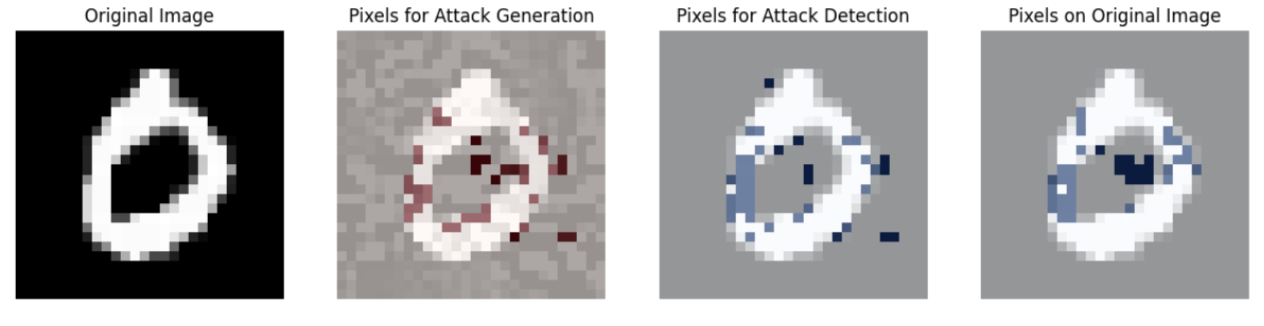
\includegraphics[width=\linewidth]{paper_images/individual.png}
        \caption{Individual Pixel Analysis. This image demonstrates the critical pixels identified in a single example, highlighting their influence on the AI model's decision-making process in response to an adversarial attack.}
        \label{fig:individual_analysis}
    \end{subfigure}
    \par\medskip % Adds space between the two subfigures
    \begin{subfigure}{.45\textwidth}
        \centering
        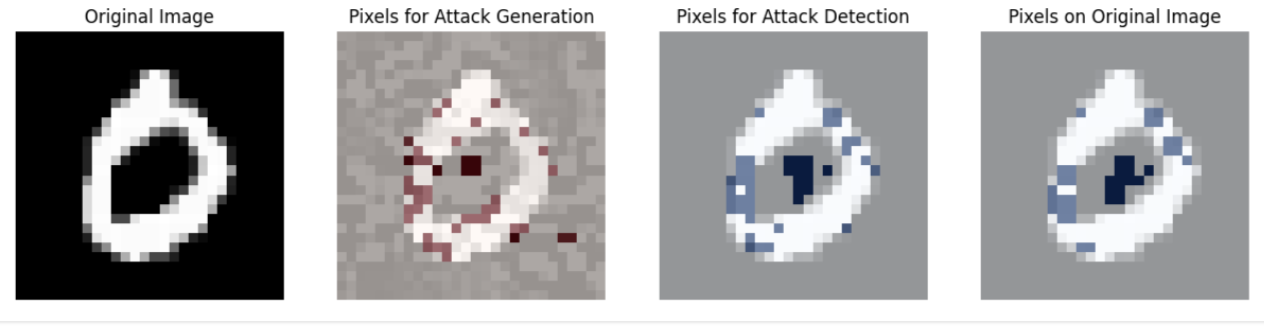
\includegraphics[width=\linewidth]{paper_images/aggregate.png}
        \caption{Aggregate Pixel Analysis. This heatmap represents the average influence of pixels across multiple examples, revealing common patterns and vulnerabilities in the AI model's interpretation of images.}
        \label{fig:aggregate_analysis}
    \end{subfigure}
    \caption{Comparative Visualization of Individual and Aggregate Pixel Analysis.}
    \label{fig:pixel_analysis}
\end{figure}

  \subsection{Case Study 3: Validation of Identified Critical Pixels}
    In Section VI, we discussed the critical pixels identified through our methodology for both attack generation and detection. To determine their significance, we conducted a rigorous statistical validation using a two-sample t-test. This validation step is crucial to highlight the critical role played by these pixels in shaping the decision-making process of our machine learning model.

    Our approach involved a comprehensive examination of SHAP values, with specific emphasis on those related to attack detection. SHAP values are useful in understanding the inner workings of our model, and they shed light on the pixels that significantly influence its predictions. To streamline the analysis, we categorized these SHAP values into two distinct groups: critical pixels and non-critical pixels. We based this categorization on a set of indices derived from our methodology.
    Figure \ref{fig:bar_chart} displays a bar chart that compares the means of two groups, highlighting the difference in mean SHAP values for 'Critical' and 'Non-Critical' pixels. This visual representation is critical to our analysis.   
    Figure \ref{fig:histograms} shows histograms of SHAP values that provide a closer look at the distribution of SHAP values for both 'Critical' and 'Non-Critical' pixels. These histograms help us to understand the data distribution and its impact on statistical tests.    
    The validation of our study primarily depends on the comparison of two groups using statistical analysis. We used the two-sample t-test, a well-known method for identifying significant differences between two sets of data. Our results were significant with a computed t-statistic of 11.5968 and an extremely low p-value of $1.34 \times 10^{-30}$. Figures \ref{fig:bar_chart} and \ref{fig:histograms} show the statistical indicators that confirm the crucial role of critical pixels in our model's behavior. These pixels influence both the generation and detection of adversarial attacks.
    
    \begin{figure*}[ht!]
        \centering
        \begin{subfigure}{.30\textwidth}
            \centering
            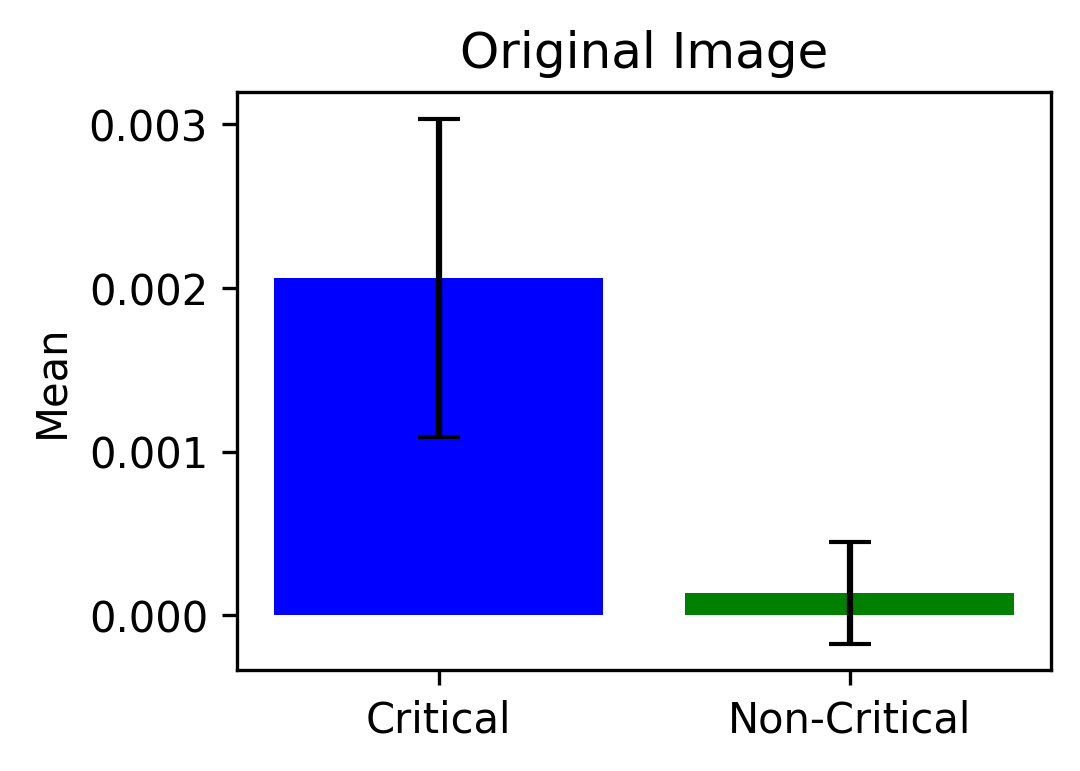
\includegraphics[width=\linewidth]{paper_images/Originalbar_chart.png}
            \caption{Original image}
        \end{subfigure}
        \begin{subfigure}{.32\textwidth}
            \centering
            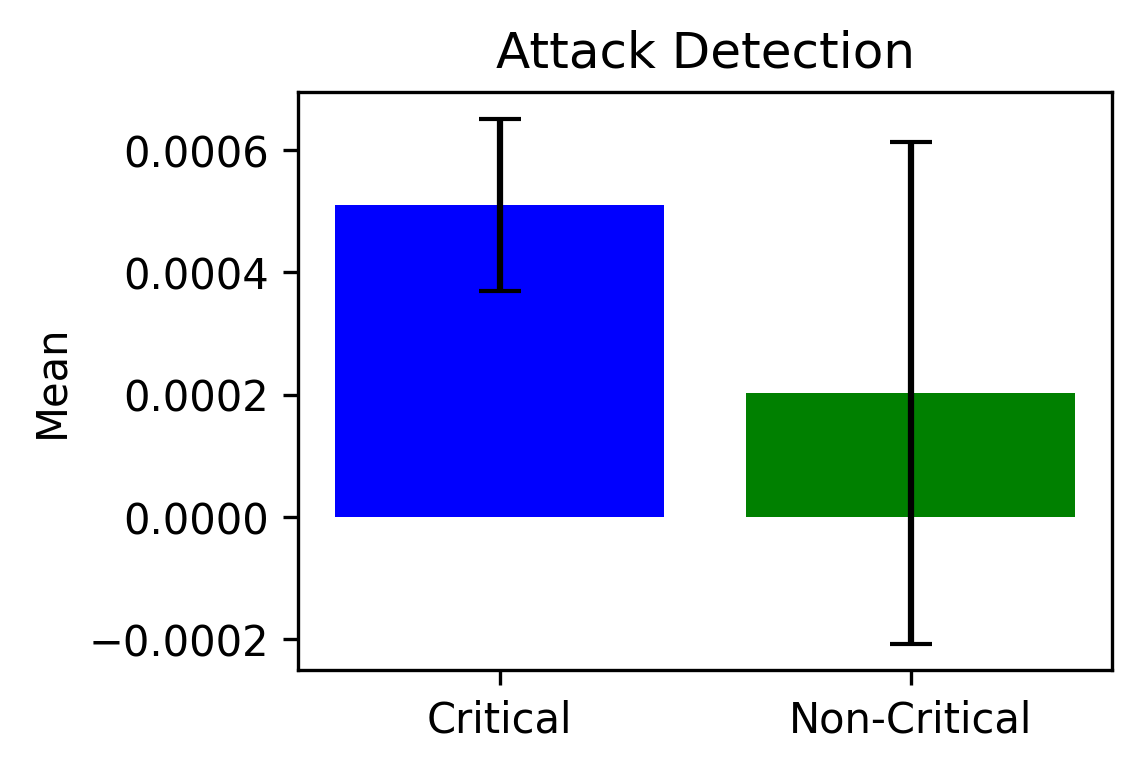
\includegraphics[width=\linewidth]{paper_images/Detectionbar_chart.png}
            \caption{Attack detection groups}
        \end{subfigure}
        \begin{subfigure}{.31\textwidth}
            \centering
            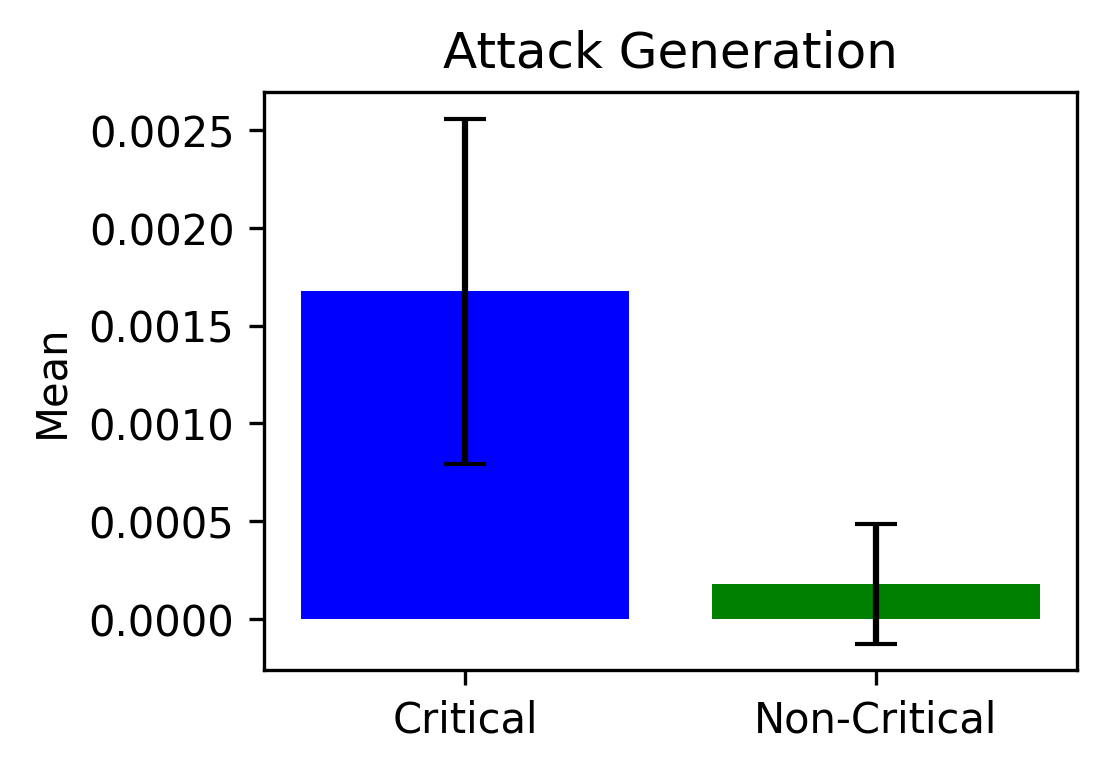
\includegraphics[width=\linewidth]{paper_images/Generationbar_chart.png}
            \caption{Attack generation groups}
        \end{subfigure}
        \caption{The bar chart illustrates a comparison between the mean SHAP values for 'Critical' and 'Non-Critical' groups. Error bars represent standard deviations. This graph is essential for assessing the significance of the differences between these groups.}
        \label{fig:bar_chart}
    \end{figure*}
    
    
    \begin{figure}[h]
        \centering
     
        \begin{subfigure}{\columnwidth}
            \centering
            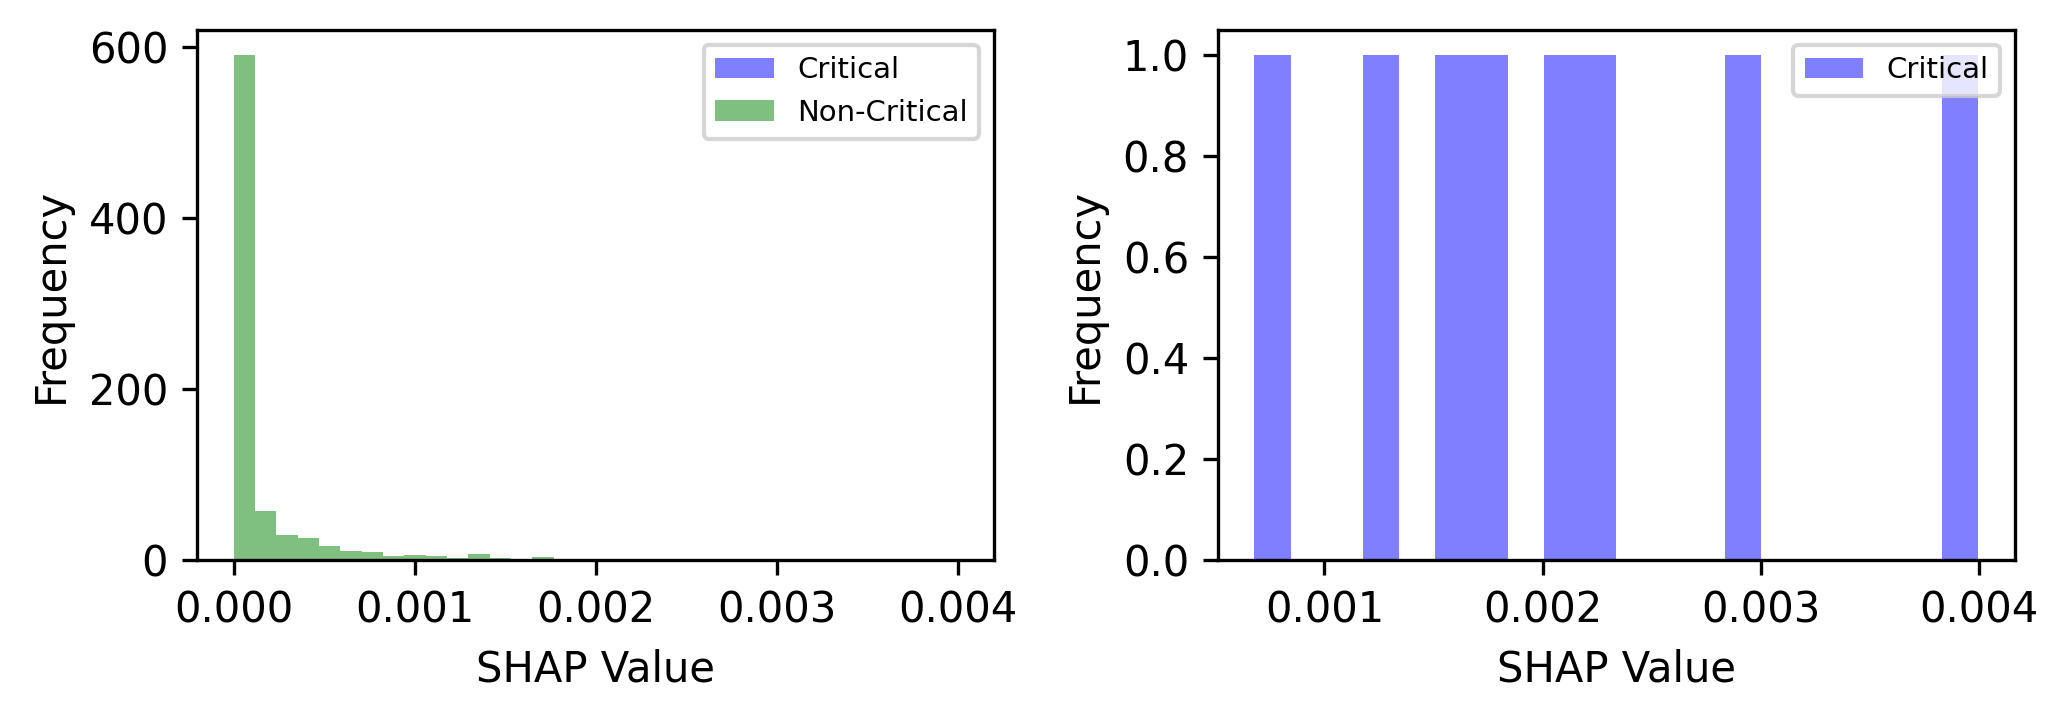
\includegraphics[width=\linewidth]{paper_images/Originalhistograms.png}
            \caption{ Orginal image for both 'Critical' (in blue) and 'Non-Critical' (in green) groups.}
           
        \end{subfigure}
        \par\medskip % Adds space between the two subfigures

        \begin{subfigure}{\columnwidth}
            \centering
            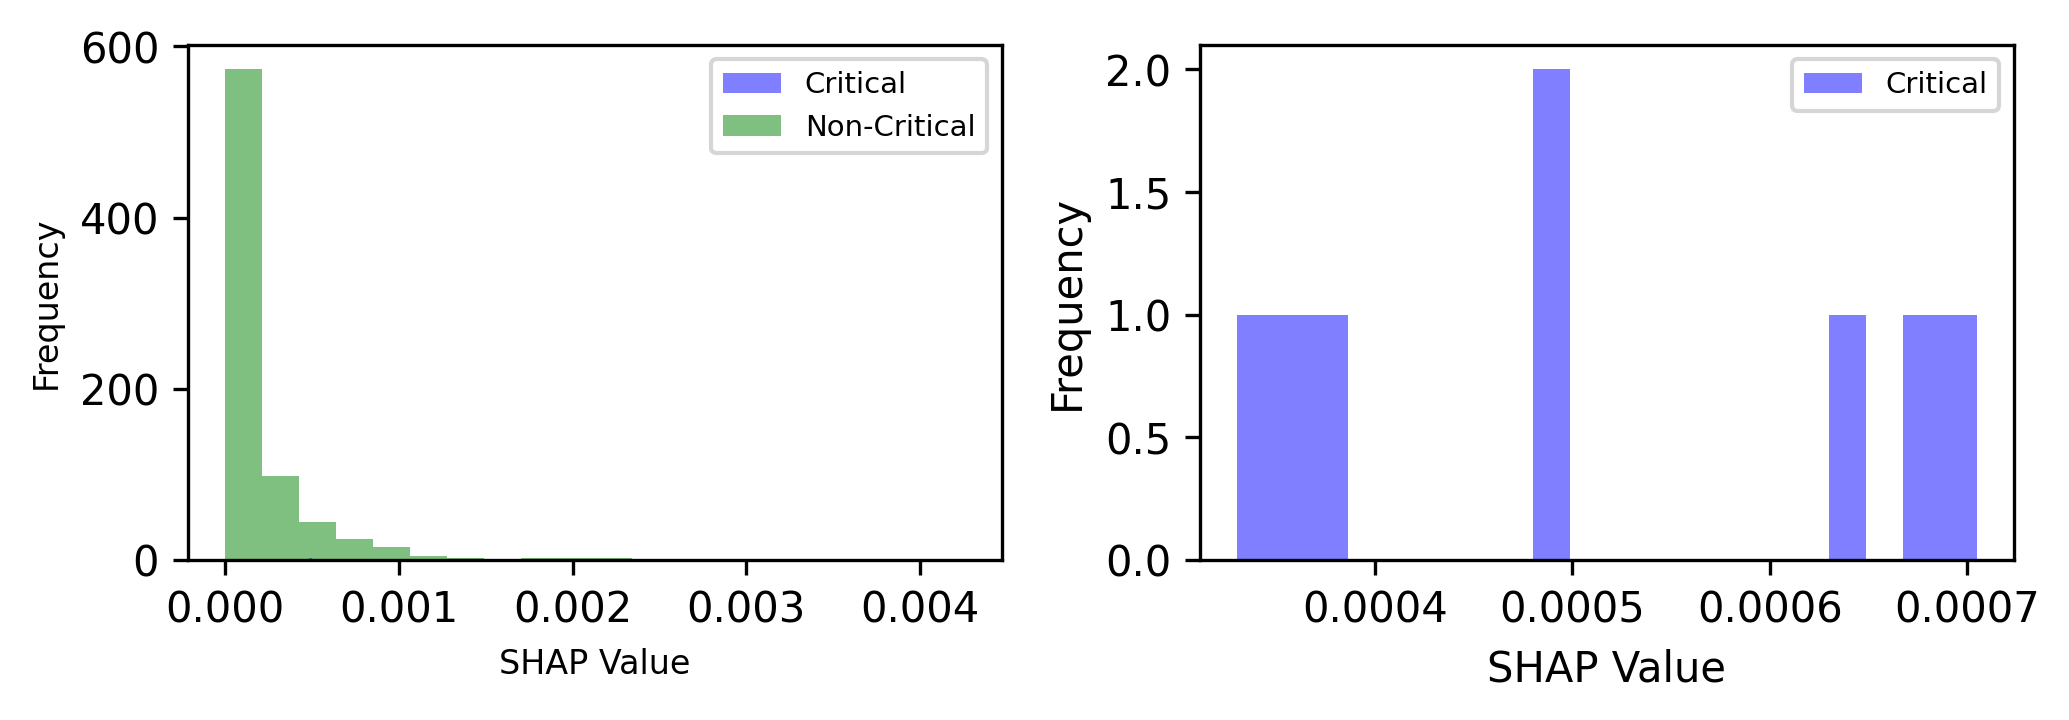
\includegraphics[width=\linewidth]{paper_images/Detectionhistograms.png}
            \caption{'Critical' (in blue) and 'Non-Critical' (in green) pixels for attack detecion group.}
        \end{subfigure}
        \par\medskip % Adds space between the two subfigures
        \begin{subfigure}{\columnwidth}
            \centering
            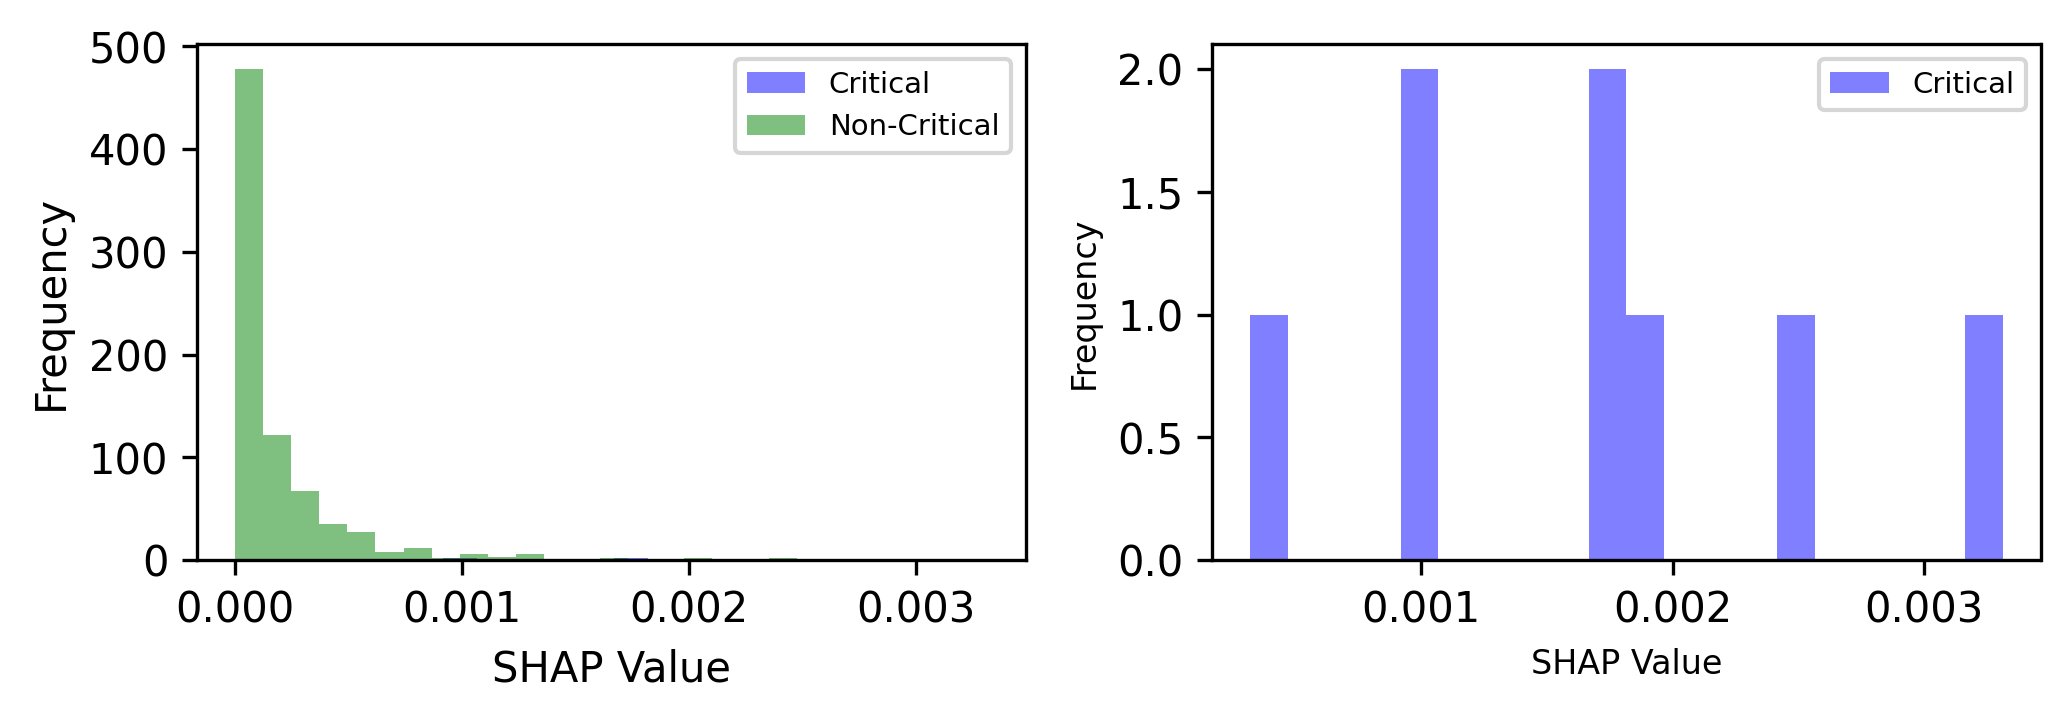
\includegraphics[width=\linewidth]{paper_images/Generationhistograms.png}
            \caption{Adversarial image for both 'Critical' (in blue) and 'Non-Critical' (in green) pixels for attack genration groups.}
          
        \end{subfigure}
        \label{fig:histograms}
        \caption{ In the left subplot, the histogram depicts the distribution of SHAP values of Adversarial image for both 'Critical' (in blue) and 'Non-Critical' (in green) groups. The right subplot zooms in on the 'Critical' group's SHAP values. These histograms provide insights into the data distribution and its impact on statistical tests}
    \end{figure}

    
% \section{Future Directions}

% By leveraging our pixel-level analysis methodology, we have identified several critical areas for future research that can extend and enhance our understanding of AI's robustness and interpretability:

% \noindent \textbf{Complex and High-Dimensional Datasets:}
% \begin{itemize}
%     \item To test the scalability and adaptability of our approach in more complex scenarios than MNIST, future research should concentrate on utilizing our pixel-level analysis on high-dimensional datasets.
%     \item This could be achieved by exploring datasets such as high-resolution medical images or real-world surveillance data.
% \end{itemize}

% \noindent \textbf{Advances in Adversarial Attack and Defense Strategies:}
% \begin{itemize}
%     \item It is necessary to develop more advanced adversarial attack techniques and defense mechanisms that are informed by pixel-level analysis.
%     \item Such developments could provide a better understanding of vulnerabilities in AI and lead to more robust AI models.
% \end{itemize}

% \noindent \textbf{Application to Various AI Architectures:}
% \begin{itemize}
%     \item Exploring the utility of SHAP analysis in various AI architectures, including RNNs and GNNs, could reveal new insights into model behavior across different domains and data types.
% \end{itemize}

% \noindent \textbf{Automated SHAP Value Analysis for Large-Scale Applications:}
% \begin{itemize}
%     \item Automated SHAP value analysis tools are critical for scaling AI applications.
% \end{itemize}

% \noindent \textbf{Cross-Domain Adaptability and Ethical Implications:}
% \begin{itemize}
%     \item Investigating the cross-domain adaptability of our approach and its ethical implications, particularly in sensitive areas like healthcare and law enforcement, would be invaluable.
%     \item This includes understanding how different stakeholders interpret and interact with SHAP-based insights.
% \end{itemize}

% \noindent Our pixel-level analysis methodology can be a foundational step for creating adaptable and trustworthy AI systems across various domains and applications.

\section{Conclusion:}
This research conducted a thorough investigation into adversarial attack simulations, analyzing the vulnerabilities of deep learning models at the pixel level. By analyzing these attacks in detail, the researchers gained insights into their intricacies. Afterwards, the power of SHAP (SHapley Additive exPlanations) analysis was used to extract Shapley values, providing a deep understanding of how each pixel contributes to model predictions. With these Shapley signatures, critical pixels within the model's decision-making process were identified. This sequential approach, starting with attack simulations, followed by Shapley analysis, and culminating in identifying critical pixels, has enriched our comprehension of adversarial threats and laid the foundation for enhancing the robustness of AI models. In conclusion, this study significantly advances our knowledge in this domain. It offers a comprehensive framework for strengthening AI models against adversarial intrusions, thereby contributing to the broader field of deep learning security.


\begin{thebibliography}{01}

    \bibitem{Saad}S. Saad, Y. Yilin, T. Haiman, T. Yudong, P. R. Maria, S. Mei-Ling, C. Shu-Ching, and S. Iyengar. "A survey on deep learning: A. Sundaraja, “ACM Computing Surveys CSUR 51 no,” 2018.
    \bibitem{Md} Z. Md, M. T. Tarek, Y. Chris, W. Stefan, S. Paheding, S. N. Mst, H. Mahmudul, C. V. E. Brian, 
    \bibitem{Numair}S. Numair, S. Ilya, and U. Mathias, “A systematic review of robustness in deep learning for computer vision Mind the gap,” 2021.
    \bibitem{Aleksandar}M. Aleksandar, S. Ludwig, T. Dimitris, and V. Adrian, “Towards deep learning models resistant to adversarial attacks,” 2017.
    \bibitem{Samuel}H. Samuel and N. Peyman, “Opportunities and challenges in deep learning adversarial robustness A survey,” 2020.
    \bibitem{Muhammad}U. Muhammad, Q. Junaid, U. J. Muhammad, A.-F. Ala, T. H. Dinh, and Niyato. "Challenges and countermeasures for adversarial attacks on deep reinforcement learning Dusit, “IEEE Transactions on Artificial Intelligence 3 no,” 2021.
    \bibitem{Mohammed}B. Mohammed, “Peeking inside the blackbox a survey on explainable artificial intelligence XAI,” 2018.
    \bibitem{Aha}Aha. "DARPA’s explainable artificial intelligence (XAI) program David, “AI magazine 40 no,” 2019.
    \bibitem{Tamer}A. Tamer, E.-S. Shaker, M. Khan, M. A.-M. Jose, C. Roberto, G. Riccardo, D. S. Javier, D.-R. Natalia, and H. Francisco, “Explainable Artificial Intelligence XAI What we know and what is left to attain Trustworthy Artificial Intelligence,” 2023.
    \bibitem{Tianhang}Z. Tianhang, Q. Zhan, and Liu. "Adversarial attacks and defenses in deep learning Xue, “Engineering 6 no,” 2020.
    \bibitem{Wei}E. Wei, Z. S. Quan, A. Ahoud, and Li. "Adversarial attacks on deep-learning models in natural language processing: A. survey Chenliang, “ACM Transactions on Intelligent Systems and Technology TIST 11 no,” 2020.

    \bibitem{ZhangS.}
    Zhang, S., Chen, S., Liu, X., Hua, C., Wang, W., Chen, K., Zhang, J. and Wang, J., 2021. Detecting adversarial samples for deep learning models: a comparative study. IEEE Transactions on Network Science and Engineering, 9(1), pp.231-244.

    \bibitem{Goodfellow.}
    I. J. Goodfellow, J. Shlens, and C. Szegedy, “Explaining and harnessing
    adversarial examples,” arXiv preprint arXiv:1412.6572, 2014.

    \bibitem{Kurakin.}A.Kurakin,I.Goodfellow,andS.Bengio,“Adversarialmachinelearning at scale,” 2016.
    \bibitem{Madry.}A. Madry, A. Makelov, L. Schmidt, D. Tsipras, and A. Vladu, “Towards deep learning models resistant to adversarial attacks,” arXiv preprint arXiv:1706.06083, 2017. 

    \bibitem{Stiff}Stiff, Harald. "Explainable AI as a Defence Mechanism for Adversarial Examples." (2019)

    \bibitem{Moosavi}S.-M. Moosavi-Dezfooli, A. Fawzi, and P. Frossard, “Deepfool: A simple and accurate method to fool deep neural networks,” in Proc.
IEEE Conf. Comput. Vis. Pattern Recognit., 2016, pp. 2574–2582.

\bibitem{Ilyas.}A. Ilyas, S. Santurkar, D. Tsipras, L. Engstrom, B. Tran, and A. Madry,
“Adversarial examples are not bugs, they are features,” arXiv preprint
arXiv:1905.02175, 2019.

\bibitem{Papernot}
N. Papernot, P. McDaniel, X. Wu, S. Jha, and A. Swami, “Distillation as a defense to adversarial perturbations against deep neural networks,” in 2016 IEEE Symposium on Security and Privacy (SP). IEEE, 2016, pp. 582–597.
\bibitem{Evans}
W. Xu, D. Evans, and Y. Qi, “Feature squeezing: Detecting adversarial
examples in deep neural networks,” arXiv preprint arXiv:1704.01155,
2017.

\bibitem{Yang} P. Yang, J. Chen, C.-J. Hsieh, J.-L. Wang, and M. I. Jordan, “ML-LOO:
Detecting adversarial examples with feature attribution,” in Proc. 34th AAAI Conf. Artif. Intell., 32nd Innov. Appl. Artif. Intell. Conf., and 10th AAAI Symp. Edu. Adv. Artif. Intell., 2020, pp. 6639–6647.
\bibitem{Feinman} R. Feinman, R. R. Curtin, S. Shintre, and A. B. Gardner, “Detecting adversarial samples from artifacts,” CoRR, 2017, arXiv: 1703.00410.
\bibitem{Ma} X. Ma et al., “Characterizing adversarial subspaces using local intrinsic dimensionality,” in Proc. Int. Conf. Learn. Representation, 2018.
\bibitem{Lee} K. Lee et al., “A simple unified framework for detecting out-of-distribution samples and adversarial attacks,” in Adv. Neural Infor. Process. Syst. 31st: Ann. Conf. Neural Infor. Process. Syst., 2018, pp. 7167–7177.

\bibitem{Ribeiro} M. T. Ribeiro, S. Singh, and C. Guestrin, “” why should i trust you?” explaining the predictions of any classifier,” in Proceedings of the 22nd ACM SIGKDD international conference on knowledge discovery and data mining, 2016, pp. 1135–1144.
\bibitem{Shrikumar} A. Shrikumar, P. Greenside, and A. Kundaje, “Learning important features through propagating activation differences,” in International conference on machine learning. PMLR, 2017, pp. 3145–3153.
\bibitem{LundbergandS} S.M.LundbergandS.-I.Lee,“Aunifiedapproachtointerpretingmodel predictions,” Advances in neural information processing systems, vol. 30, 2017.

\bibitem{Singh} A. Singh, S. Sengupta, and V. Lakshminarayanan, “Explainable deep learning models in medical image analysis,” Journal of Imaging, vol. 6, no. 6, p. 52, 2020.

\bibitem{Mangalathu} S. Mangalathu, S.-H. Hwang, and J.-S. Jeon, “Failure mode and effects analysis of rc members based on machine-learning-based shapley addi- tive explanations (shap) approach,” Engineering Structures, vol. 219, p. 110927, 2020.

\bibitem{Aouf}L. He, N. Aouf, and B. Song, “Explainable deep reinforcement learning for uav autonomous path planning,” Aerospace science and technology, vol. 118, p. 107052, 2021.
\bibitem{Parsa} A. B. Parsa, A. Movahedi, H. Taghipour, S. Derrible, and A. K. Mohammadian, “Toward safer highways, application of xgboost and shap for real-time accident detection and feature analysis,” Accident Analysis \& Prevention, vol. 136, p. 105405, 2020.
\bibitem{Huang}  H. Wu, A. Huang, and J. W. Sutherland, “Layer-wise relevance prop-
agation for interpreting lstm-rnn decisions in predictive maintenance,” The International Journal of Advanced Manufacturing Technology, vol. 118, no. 3, pp. 963, 2022.

\bibitem{Warnecke} A. Warnecke, D. Arp, C. Wressnegger, and K. Rieck, “Evaluating explanation methods for deep learning in security,” in 2020 IEEE european symposium on security and privacy (EuroS\&P). IEEE, 2020, pp. 158.

    \bibitem{McInnes.}
	L. McInnes, J. Healy, and J. Melville, “UMAP: Uniform Manifold Approximation and Projection for Dimension Reduction,” ArXiv e- prints, Feb. 2018.
  
 
\end{thebibliography}

\end{document}
